%% Single-page style
\documentclass[12pt,a4paper]{report}
\setlength\textwidth{145mm}
\setlength\textheight{247mm}
\setlength\oddsidemargin{15mm}
\setlength\evensidemargin{15mm}
\setlength\topmargin{0mm}
\setlength\headsep{0mm}
\setlength\headheight{0mm}

\let\openright=\clearpage  % macro - what follows starts on the right page

%% Both-pages style
% \documentclass[12pt,a4paper,twoside,openright]{report}
% \setlength\textwidth{145mm}
% \setlength\textheight{247mm}
% \setlength\oddsidemargin{15mm}
% \setlength\evensidemargin{0mm}
% \setlength\topmargin{0mm}
% \setlength\headsep{0mm}
% \setlength\headheight{0mm}
% \let\openright=\cleardoublepage

\usepackage[utf8,utf8x]{inputenc}

\usepackage[english]{babel}
\usepackage{graphicx}
\usepackage{booktabs}
\usepackage{natbib}
\usepackage{mathptmx}
%\usepackage[charter]{mathdesign}
\bibpunct{(}{)}{;}{a}{,}{,}
\usepackage{ucs}
\usepackage{setspace}

\usepackage{amsmath}
\usepackage{amsfonts}
\usepackage{amssymb}
\usepackage{tikz}
\usepackage{booktabs}

\DeclareMathOperator*{\argmax}{arg\,max}

\usepackage[hyphens]{url}
\usepackage[unicode]{hyperref}   % Musí být za všemi ostatními balí�?ky
\hypersetup{
    unicode=true,          % non-Latin characters in Acrobat’s bookmarks
    pdftitle={todo},    % title
    pdfauthor={todo},     % author
    pdfsubject={todo},   % subject of the document
    pdfcreator={todo},   % creator of the document
    pdfkeywords={todo}, % list of keywords
    pdfstartview={FitH},   %fit horizontally
    colorlinks=true,       % false: boxed links; true: colored links
    linkcolor=black,          % color of internal links
    citecolor=black,        % color of links to bibliography
    filecolor=black,      % color of file links
    urlcolor=blue           % color of external links
}

\newcommand{\todoa}[1]{[\textbf{TODOA} #1]}
\newcommand{\todob}[1]{[\textbf{TODOB} #1]}
\newcommand{\todoc}[1]{[\textbf{TODOC} #1]}

\newcommand{\e}[1]{\textit{#1}} % language expressions, examples

%%% Small modifications
%
% Tato makra přesvěd�?ují mírně ošklivým trikem LaTeX, aby hlavi�?ky kapitol
% sázel pří�?etněji a nevynechával nad nimi spoustu místa. Směle ignorujte.
%\makeatletter
%\def\@makechapterhead#1{
%  {\parindent \z@ \raggedright \normalfont
%   \Huge\bfseries \thechapter. #1
%   \par\nobreak
%   \vskip 20\p@
%}}
%\def\@makeschapterhead#1{
%  {\parindent \z@ \raggedright \normalfont
%   \Huge\bfseries #1
%   \par\nobreak
%   \vskip 20\p@
%}}
%\makeatother

% Non-numbered chapter, present in TOC
\def\chapwithtoc#1{
\chapter*{#1}
\addcontentsline{toc}{chapter}{#1}
}
\usepackage{covington}


\begin{document}

% hyphenation
\lefthyphenmin=2
\righthyphenmin=2


%%% Title page

\pagestyle{empty}
\begin{center}

\large

Charles University in Prague

\medskip

Faculty of Mathematics and Physics

\vfill

{\bf\Large MASTER'S THESIS}

\vfill

\centerline{\hspace{18mm}\mbox{
\includegraphics[width=60mm]{logo.pdf}}}

\vfill
\vspace{5mm}

{\LARGE Sr\dj an Prodanovi\'{c}}

\vspace{15mm}

% NAME
{\LARGE\bfseries  Word Sense Disambiguation\\ in Prague Dependency Treebank\\ via Distributional Semantics Approach}

\vfill

Institute of Formal and Applied Linguistics
\vfill

\begin{tabular}{rl}

Supervisor of the master's thesis: &  RNDr.~Ji\v{r}\'i Hana, Ph.D., \\
					&	Institute of Formal and Applied Linguistics\\
\noalign{\vspace{2mm}}
Study programme: & Computer Science\\
\noalign{\vspace{2mm}}
Specialisation: & Computational and Formal Linguistics\\
\end{tabular}

\vfill

Prague 2012

\end{center}

\newpage


\openright
\onehalfspacing
\noindent
At a very high risk of sounding extremely clich\'ed I do have to say that I am profoundly grateful for the chance of being exposed to such exciting areas of CL and NLP. The decision to take the the two years off work and attend this program was (unintentionally) one of the best decisions of my life. Of course I would not be able to struggle all the challenges without the constant support of my family, my love  and my friends. I also wish to thank all the wonderful people from the program, both teachers and colleagues for equally helping me thrive in the areas of my interest. Lastly I wish to thank the Erasmus Mundus organization for supporting the LCT program and giving  a chance to non--European students to attend truly excellent studies.


\newpage

%%% Strana s �?estným prohlášením k diplomové práci

\vglue 0pt plus 1fill

\noindent
I declare that I carried out this master's thesis independently, and only with the cited sources, literature and other professional sources.

\medskip\noindent
I understand that my work relates to the rights and obligations under the Act No. 121/2000 Coll., the Copyright Act, as amended, in particular the fact that the Charles University in Prague has the right to conclude a license agreement on the use of this work as a school work pursuant to Section 60 paragraph 1 of the Copyright Act.

\vspace{10mm}

\hbox{\hbox to 0.5\hsize{%
In ........ date ............
\hss}\hbox to 0.5\hsize{%
signature
\hss}}

\vspace{20mm}
\newpage

%%% Povinná informa�?ní strana diplomové práce
\singlespacing
\vbox to 0.5\vsize{
\setlength\parindent{0mm}
\setlength\parskip{5mm}

Název práce:
 Word Sense Disambiguation in Prague Dependency Treebank via Distributional Semantic Approach
% přesně dle zadání

Autor: Sr\dj an Prodanovi\'{c}

Katedra: \'Ustav form\'aln\'i a aplikovan\'e lingvistiky (UFAL)

Vedouc\'{i} diplomov\'{e} pr\'{a}ce:
 RNDr.~Ji\v{r}\'i Hana, Ph.D., Institute of Formal and Applied Linguistics

\onehalfspacing
Abstrakt:
In statistical models of semantics word meanings are based solely on their distributional properties. 
The core resource here is a single lexicon that can be used for a variety of tasks, where word meanings are represented as vectors in Vector Space, and word 
similarities as distances between their vector representations. Using strengths of similarities, appropriateness of terms given a 
particular context can be calculated and used for a variety of tasks, one of them being Word Sense Disambiguation.
\newline
In this thesis several different approaches to models of Vector Space were examined and implemented in order to cross 
evaluate their performance on the Word Sense Disambiguation task in Prague Dependency Treebank. 

Kl\'{i}\v{c}ov\'{a} slova:
word sense disambiguation, vector space model, prague dependancy treebank
\onehalfspacing
\vss}\nobreak\vbox to 0.49\vsize{
\setlength\parindent{0mm}
\setlength\parskip{5mm}

Title:
Word Sense Disambiguation in Prague Dependency Treebank via Distributional Semantic Approach

Author:
Sr\dj an Prodanovi\'{c}

Department:
Institute of Formal and Applied Linguistics
% dle Organiza�?ní struktury MFF UK v angli�?tině

Supervisor:
RNDr.~Ji\v{r}\'i Hana, Ph.D., \'Ustav form\'aln\'i a aplikovan\'e lingvistiky

\onehalfspacing
Abstract:
In statistical models of semantics word meanings are based solely on their distributional properties. 
The core resource here is a single lexicon that can be used for a variety of tasks, where word meanings are represented as vectors in Vector Space, and word 
similarities as distances between their vector representations. Using strengths of similarities, appropriateness of terms given a 
particular context can be calculated and used for a variety of tasks, one of them being Word Sense Disambiguation.
\newline
In this thesis several different approaches to models of Vector Space were examined and implemented in order to cross 
evaluate their performance on the Word Sense Disambiguation task in Prague Dependency Treebank. 

Keywords:
word sense disambiguation, vector space model, prague dependancy treebank
\vss}

\newpage


%% TOC
\onehalfspacing
\openright
\pagestyle{plain}
\setcounter{page}{1}
\tableofcontents

%\chapter*{Introduction}
\chapter{Introduction}

\begin{section}{About the task}
Lexical disambiguation is concerned with determining the meaning of every word given their context. As a computational problem it is often described as "AI--complete", which means that in order to solve the problem of word meaning one needs to solve completely  natural--language understanding or common-- sense reasoning (Ide and V\'eronis 1998)
%\cite{nancy1998}
. Fortunately, this is in not the case in the field of computational linguistics. There, this problem is generally called word sense disambiguation (WSD), and is defined as the problem of computationally determining which ``sense'' of a word is activated within a particular context. WSD is essentially a task of classification: word senses are the classes, a word's context contains necessary disambiguation information, and each occurrence of a word is assigned to one or more of its possible classes depending on the context information.
\newline
\newline The Prague Dependency Treebank is a large annotated corpus built to further the research in Computational Linguistics for Czech language. It is fully annotated at morphological and syntactic analytic  layers of annotation as well as in tectogrammatical layer. Like any other language, Czech language has its own share of words with multiple meanings. Thus the main task of this thesis is word sense disambiguation on PDT dataset. 
\end{section}
\section{About the model} \label{aboutTheModel}
Semantic theory has existed long enough to witness many different attempts to represent the meaning of 
words. Starting from Frege, Tarsky and Davidson's Propositional Logic representations where they 
concentrated 
on the Propositions about Symbols, calculating the ``truth'' of those Propositions. However, they were more 
focused on ``truth conditions''  and less on the content (representing what the propositions are about). (De 
Saussure 1878) 
%\cite{SAUSSURE_1878} 
 in his first work talks about the \textit{signifier} (the signs) and the \textit{signified} (the "meaning"), 
followed with the theory of mediated reference (Frege 1892)
%\cite{frege1892} 
where he makes a distinction between
sense (intension) and reference (extension). Then comes the theory of direct reference (Rusell 1905)
%\cite{rusell1905} 
who equates the meaning with reference. If we look even further in history and beyond linguistic theory we 
can find examples in philosophy like with Aristotle where he describes concepts as a finite sets of features 
that belong to different categories (animate--inanimate, etc.). Leibnitz also used this approach when he tried 
to make his "language of meaning".
\\\\ 
 \textbf{Some applications.} A large part of Natural Language Processing today is concerned with tasks and applications related to the use of meaning, like  lexicon acquisition, word--sense disambiguation, information access, machine translation, dialogue systems, etc. Vector space models have proven to be applicable in these fields. 
Another immediate application could be in the field of Information Retrieval, in particular for the expansion of user queries, since word--space models easily retrieve nearest neighbours in semantic space,  in order to obtain better search results. 
%\todo{perhaps this should be left for "future work" section?}
\newline
\newline \textbf{Intuitiveness.}
There is a certain intuitiveness behind statistical models of semantics. Experiments by Tom Mitchell\cite{mitchell2008} successfully predict the fMRI (fuctional MRI) brain images for particular nouns, based on fMRI images of seen nouns, completely relying on statistical approach. Lexical priming studies beginning with Ratcliff \& McKoon (1978)
%\cite{ratcliff1978}
 and Swinney (1979)
%\cite{swinney1979lexical} 
as well as eye movement studies (Rayner, Pacht, \& Duffy, 1994)
%\cite{raynerPacht1994}
, suggest that ambiguous words first activate multiple interpretations, but very soon settle to that sense most appropriate to their discourse contexts. An analogy to estimating the amount of appropriateness of a word's meaning in some context could be drawn to the same way the scores of a word's meaning in some context are calculated, as will be presented in this thesis. It should  be noted that computational models presented here are not necessarily similar to the way humans process information when they think about word meaning. They are however empirically consistent with human behaviour when they are performing semantic related tasks. 

\section{Thesis goals}   
Main goal of this Master's thesis is to, by utilizing various approaches to statistical representation of 
semantics, perform a Word Sense Disambiguation using Prague Dependency Treebank as a dataset. 
Various approaches that were used for the task utilize different statistical models of semantics, and they as well as subsume a variety of steps in linguistic and statistical preprocessing of text. All necessary parameters
are tuned in order to achieve best results for every model examined. Therefore, the secondary goal of this thesis was to establish the methodology by which preprocessing steps and tuning of models parameters should occur. 

\section{Road map}
This thesis is organized as follows: second chapter is describing the Word sense disambiguation task, its 
purpose, applications and overview of approaches. Next chapter explains the statistical model of 
 semantics starting from motivation, rationale and then details the mathematical foundation of 
word--space models. Chapter after that is devoted to the problem of high dimensionality, present in
word--space models, and gives an overview of best known techniques in overcoming this issue. Chapter
four describes all the steps that can be taken when constructing the model, concentrating on presenting current approaches to such steps. With chapter four the theoretical part of the thesis is concluded. Chapter five, which is on experiments, details all the steps taken in experiments performed. Here are described: the research methodology and sections devoted to presenting tuning and results for three word--space models
used for WSD task. Final chapters describe the implementation and in the user manual explain how the 
implementation should be run when performing experiments.

%\addcontentsline{toc}{chapter}{Introduction}


\chapter{Computational model of semantics}
The computational model of semantics presented here is referred to in the literature as the \textit{word--space model} or \textit{vector--space model} (VSM). Term was coined by Hinrich Sch\"{u}tze (1993) who defined the model as:
\begin{quotation}\textit{Vector similarity is the only information present in Word Space: semantically related words are close, unrelated words are distant. (p.896)}
\end{quotation}

\section{Motivation}
Despite the wealth of theories on meaning only a number of them has proven to be fully functional in an actual implementation. This is mainly due to the fact that linguistic data tends to be variable, inconsistent and vague. Keeping this in mind, a categorization of approaches can be viewed (Jurafsky, Martin 2000):
\begin{enumerate}
\item Representational approach: involves the creation of formal \textbf{meaning representations} that are intended to bridge the
gap from language to commonsense knowledge of the world. These representations need to be able to support the practical aspects of semantic processing, like to resolve the truth of propositions, to support unambiguous representations,
to represent variables, and to support inference. Human languages have various tools used to convey meaning, the most important being the one used to convey a \textbf{predicate--argument structure}. First order Predicate Calculus is a computationally tractable
meaning representation language that is used mainly for the purpose of handling predicate--argument structure. 
\item Syntax-driven approach: rests on the \textbf{Principle of Compositionality} that states that the meaning of a sentence can
be composed from the meanings of its parts. Semantic analyzers that make use of static knowledge from the lexicon and
grammar can create context-independent literal, or conventional, meanings. In Syntax-driven semantic analysis, the parts are the syntactic constituents
of an input.
%\item Prescriptive approach: language is viewed as ambiguous and incomplete. It is therefore recommended to have a more exact form of a language model that will make up for all the shortcomings of language. Language should be modeled in abstract. 
%\item Descriptive approach: believe that ambiguity, vagueness and incompleteness do not represent a malfunctions of language and should therefore not be forced into a single formalism.   
\end{enumerate}
Vector--space models described in this thesis rely completely on the language data and do not have a single rule or constraint pre--written 
into the model.
Apart from the advantage of avoiding laborious task of handcrafting rules for the model of semantics, 
statistical modeling has yet another advantage- its construction is entirely automatic, straight from the
raw or annotated corpus. Since the modeling depends on the data set used in training, results are completely optimized toward that data set.

\section{Similarity is proximity}
The word--space model is a spatial representation of a word meaning. If every word is represented as a vector in n--dimensional space then the claim is that semantic (un)similarity of those words can be measured as a distance between their vectors. To illustrate this on a simple example for vectors representing meanings of 2 words in 2--dimensional space:

\setlength{\unitlength}{5cm}
\begin{picture}(1,1)
\put(0,0){\line(0,1){1}}
\put(0,0){\line(1,0){1}}
\put(0.75,0.75){$tangerine$}
\put(0,0){\vector(1,1){0.75}}
\put(0.5,0.2){$orange$}
\put(0,0){\vector(3,1){0.5}}
\end{picture}
\\\\
Semantic similarity between words can be measured as a distance between vectors representing \textit{tangerine} and \textit{orange}. Mathematical background of this claim will be explained in detail later in chapter 5.5.
\\\\  Distance in space as a way to represent semantic similarity seems to be a very natural and intuitive idea. This has been pointed out in a number of works by George Lakoff and Mark Johnson (Lakoff \& Johnson, 1980, 1999)
 where it is explained how humans use their spatio--temporal knowledge to conceptualize abstract objects.
(Sahlgren 2006)
 notes that \textit{similarity--is--proximity} also entails another geometric metaphor: \textit{concepts--are--locations}. This is also important to observe because in Distributional Semantics word meanings are percieved according to the differential property of their geometric locations in the Word Space. 

\section{Distributional manifestation of meaning}
In the word--space model similarities between words are automatically extracted from language data. As data, the word--space model uses statistics about the distributional properties of words. (Sahlgren 2006) has formulated from this insight his \textit{Distributional Hypothesis} which states:
\begin{quotation}
\textit{Words with similar distributional properties have similar meanings.}
\end{quotation}
There are number of examples in previous work to back this claim. (Schutze \& Pedersen 1995), claim that  ''words with similar meanings will occur with similar neighbors if enough text material is available", and (Rubenstein \& Goodenough 1965) in one of the very first studies to explicitly formulate and investigate the distributional hypothesis state that  "words which are similar in meaning occur in similar contexts" .

According to Zelig Harris in his "Mathematical Structures of Language" linguistic meaning is inherently 
differential, instead of referential which means that differences in meaning are visible through the 
differences in distribution. One of the first experiments to back this is (Rubenstein \& Goodenough 1965), who compared contextual similarities with synonymy judgments provided by university students. Their experiments demonstrated that there indeed is a correlation between semantic similarity and the degree of contextual similarity between words.

\section{Context vectors}
After describing the geometrical intuition behind the semantic similarity in this section will be explained how the model is built. Let us start by quoting Zelig Harris:
\begin{quotation}
The distribution of an element will be understood as the sum of all its environments. (Z. Harris, 1970, p.775)
\end{quotation}

Let us illustrate on a one sentence example how a distributional model could be built from it: 
\begin{quotation}
"Where there is smoke there is fire."
\end{quotation}
We start by determining what is the appropriate environment of the word. In linguistics word environment is called \textbf{context}. In our example we will restrict the context to the preceding and succeeding word. Distributions gathered from our example are shown in the table below. 
\\
\begin{center}
\begin{tabular}{ l | c c c c c }
   &  where & there & is & smoke & fire\\
  \hline                       
  where & 0 & 1 & 0 & 0 & 0 \\
  there & 1 & 0 & 2 &  0 & 0 \\
  is & 0 & 2 & 0 & 1 & 1 \\
  smoke & 0 & 0 & 1 & 0 & 0 \\
  fire & 0 & 0 & 1 & 0 & 0 \\
\end{tabular}
\end{center}
As we can see from the table every word is represented with a vector, for instance "smoke" is (0,0,1,0,0). To put it more formally: every vector is defined by \textit{n} components, where each component represents a location in n--dimensional space. To quote Magnus Sahlgren's definition on context vectors:
\begin{quotation}
I call the co--occurrence counts \textit{context vectors} because they effectively constitute a representation of the sum of the word's contexts.
\end{quotation} 

\subsection{A brief history of context vectors}
The notion of context vectors has begun with the prominent work in psychology by Charles Osgood in the 1950's on feature space representations of meaning, which he called \textit{semantic differential approach to meaning representation}. In this approach words are represented as feature vectors where elements are contrastive adjective pairs such as "soft--hard", fast--slow", etc. The idea was to measure the psychological difference between words. An example from the research is given below. 

\begin{table}[h!]
\begin{center}
\begin{tabular}{ l | c c c  }
   &  small--large & bald--furry& docile--dangerous\\
  \hline                       
  mouse & 1 & 6 & 1\\
  rat & 2 & 6 & 4 \\
\end{tabular}
\caption{Feature vectors based on three contrastive pairs for words mouse and rat}
\end{center}
\end{table}
Osgood's work was an inspiration for Stephen Gallant, who introduced the term "context vector" to
describe the feature--space representations (Gallant, 1991a). In Gallant's algorithm, context vectors were defined with a set of manually derived features, such as "human, "man, "machine," etc. However as some researchers later noticed drawbacks of this approach to describe the word's semantics were:
\\1. which features should be used?	
\\2. how many features are enough?
\\\\  These questions led to first approaches to \textit{automatically} construct a feature space. One of the first approaches was by Gallant (1991b) where he described the algorithm in two steps:
\begin{enumerate}
\item A context vector is initialized for each word as a normalized random vector.
\item While making several passes through the corpus, the context vectors are changed to be more like the context vectors of the surrounding words.
\end{enumerate}
The results were then used for word--sense disambiguation, where he calculated meanings for words from context, and compared them to the manually defined ones (Gallant, 1991b). However, probably the most influential work comes from Hinrich Sch\"utze (1992, 1993), who built context vectors (which he calls "term vectors" or "word vectors") similarly to the approach described above: co--occurrence counts are collected in a words--by--words matrix, in which the elements record the number of times two words co--occur within a set window of word tokens. Context vectors are then defined as the rows or the columns of the matrix.
%\\\\  Not all attempts are oblivious to the notion of grammar though. There were also some grammar--informed methods as well. Lin (1998) measures similarity of any two things (words, documents, people, plants) as a function of the information gained by having: a joint description of \textit{a} and \textit{b} in terms of what they have in common compared to describing \textit{a} and \textit{b} separately. For instance, do we gain more by a joint description of:
%\begin{enumerate}
%\item apple and chair (both THINGS)

%\item apple and banana (both FRUIT: more specific) 
%\end{enumerate}


\section{The co--occurrence matrix} \label{coOcMatrix}
The most formal definition of a co--occurrence matrix would be that it is a matrix of co--occurrence counts of its elements. The matrix can be a words--by--words matrix \textit{w} $\times$ \textit{w}, where w are the word types in the data, or a words--by--documents matrix \textit{w} $\times$ \textit{d}, where d are the documents in the data. A cell $f_{ij}$ of the co--occurrence matrix contain the frequency of occurrence of word \textit{i} in the context of word \textit{j} or in document \textit{j}, depending on the matrix type.
\\In the study on Vector Space Models of Semantics (Turney\&Pantel, 2010) authors look into various approaches to the task of  semantic processing of text. They observe and classify Vector Space Models into three main classes, depending on the type of the co--occurrence matrix they are based on: term--document, word--context or pair--pattern matrices. 

\begin{enumerate}
\item \textbf{Term--Document matrix:} The row vectors of the matrix correspond to terms (usually 
terms are words, but there are also other possibilities), and the column vectors correspond to 
documents (web pages, for example).  Term--Document matrix follows the "bag--of--words" hypothesis, 
which means that the order of words does not matter in order to estimate the importance of the query 
to the document (Salton et al. 1975). The "bag" here is like a mathematical set, with 
allowed duplicates.  To illustrate this on a simple example using pseudo--words: bag \{aa, ab, aa, ab, 
ac\} contains elements aa, ab, ac. The order of bag's elements is of no relevance here-- bag \{aa, ab, 
aa, ab, ac\} is the same as a bag \{aa, aa, ab, ab, ac\}. If we measure raw frequencies, this bag can 
be represented with a vector \textbf{A}=\{2,2,1\} where first element is the frequency of \textit{aa}, 
second element is the frequency of \textit{ab}, and third element is the frequency of \textit{ac}. A set of 
bags can be represented as a matrix X, in which each column $x_{:j}$ corresponds to a bag, each row 
$x_{i:}$ corresponds to a unique term, and an element $x_{ij}$ is the frequency of the \textit{i}--th 
term in the \textit{j}--th bag. If we look at the documents as bags, this example is easily transported into the 
Information Retrieval domain. The pattern of numbers in $x_{i:}$ is a kind of signature of the i--th term 
$w_{i}$; likewise, the pattern of numbers in $x_{:j}$ is a signature of the \textit{j}--th document 
$d_{j}$. This means that the pattern of numbers reveal, to some degree, what the term or document is 
about.

The vector does not attempt to capture the structure in the phrases, sentences, paragraphs, and 
chapters of the document. Despite this omission, search engines work really well when based on term 
document matrix. Term--document matrix reflects in fact the similarity of documents. In the IR domain, 
search engines treat queries as documents, and return search results whose score is based on the degree of similarity 
between query vectors and all document vectors in corpus.
\item \textbf{Word--Context matrix:} Deerwester et al. (1990) observed 
that we can shift the focus to measuring word similarity, instead of document similarity, by looking at 
row vectors in the term--document matrix, instead of column vectors. In general, we may have a 
word--context matrix, in which the context is given by words, phrases, sentences, paragraphs, chapters 
or documents. A word may be represented by a vector in which the elements are derived from the 
occurrences of the word in various contexts, such as windows of words (Lund \& Burgess, 1996), 
grammatical dependencies (Lin, 1998), and richer contexts consisting of dependency links 
and selectional preferences on the argument positions (Erk \& Pad\'o, 2008). To 
illustrate this on a simple example: consider a co--occurrence matrix populated by simple frequency 
counting: if word \textit{i} co--occurs 16 times with word \textit{j}, we enter 16 in the cell $f_{ij}$ in 
the words--by--words co--occurrence matrix. The co--occurrences are normally counted within a 
context window spanning some (usually small) number of words.

\item \textbf{Pair-- Pattern Matrix:} reflects the similarity of relations. Row vectors correspond to pairs of words, such as \textit{mason : stone} and \textit{carpenter : wood}, and column vectors correspond to the patterns in which the pairs co--occur, such as \textit{"X cuts Y"} and \textit{"X works with Y"}. Turney et al. (2003) introduced the use of the pair--pattern matrix for measuring the semantic similarity of relations between word pairs, which in this case is the similarity of row vectors. The \textit{latent relation hypothesis} is that pairs of words that co--occur in similar patterns tend to have similar semantic relations (Turney, 2008a). Word pairs with similar row vectors in a pair--pattern matrix tend to have similar semantic relations.
\end{enumerate}

(Sch\"utze and Pedersen 1993) defined two ways that words can be 
distributed in a corpus of text: If two words tend to be neighbours with each other, then they are 
syntagmatic associates. If two words have similar neighbours, then they are paradigmatic parallels. As 
they noted, syntagmatic associates are often different parts of speech, whereas paradigmatic parallels 
are usually the same part of speech. Syntagmatic associates tend to be semantically associated (for 
example, bee and honey), while paradigmatic parallels tend to be taxonomically similar (for example 
doctor and nurse ).
\\\\  While word--document and word--word matrices reflect attributional relations between word 
senses, the pair--pattern matrix reflects relational similarity between word senses. This distinction was 
explained in (Gentner 1983). Being that we are focused in this dissertation on the 
application of vector space models solely on the task of WSD we are interested only in models that stem 
from attributional kind of relationship, thus utilizing the first two kinds of matrices. The pair--pattern 
matrix has proven track record with other applications, for example one of them being the analogies 
task, and is therefore of no interest to implement in this research.
\chapter{Word sense disambiguation}
\section{Word sense(s)}
A meaning of a word is a variable category, very much dependent on its surrounding context. In the field 
of lexical semantics it is found that many words have overlapping or extended meanings (Kilgarriff 
1997). ''Polysemy" of a word means that it has multiple, but related meanings. At a 
more coarse grained level of meaning words that have the same spelling and pronunciation as each other but different meanings and origins are called \textit{homonyms}. Polysemy is a 
feature of words while ''ambiguity" is a property of text. If there is uncertainty about  the meaning of a 
word there is ambiguity about the whole text as well. 
Probably the most well known example of an ambiguous word is the word \textit{bank}, which contains
two homonyms: as a  as financial institution, and as a river bank. Bank as financial institution splits 
further into the following cloud of related senses: the company or institution, the building itself, the 
counter where money is exchanged, a fund or reserve of money, a money box (piggy bank), the funds in 
a gambling house (WordNet 2.1)\footnote{http://wordnet.princeton.edu/}.
Different words have different number of meanings.
A view on the number of senses word might have is somewhat controversial. Some argue that task--
independent senses simply cannot be enumerated in a list (Kilgarriff 1997) while 
others claim that words can have only a single, abstract meaning (Ruhl 1989).
\newline
\newline 
WSD was first formulated as a distinct computational task during the early days of machine translation. It was Weaver
 (1949) who noted in his memo on machine translation the importance of context in determining word sense(s), by conducting a simple experiment- observing words from a sentence in isolation, and trying to determine their meaning. (Zipf 
1949) published his "Law of Meaning"  where he states  that more frequent words 
have more senses than less frequent words in a power--law relationship. A valuable point worth noting 
in any experiment with WSD. This was later confirmed for the British National Corpus (Edmonds 2005) 
 as well.
\\\\  
Statistical and machine learning methods have been successfully applied to the WSD problem. Methods that train on manually sense--tagged corpora (like Penn Treebank, or Prague Dependency Treebank) are called supervised learning methods. Since models implemented in this thesis are trained on annotated corpus, they are as well supervised. Supervised methods have become in general the mainstream approach to WSD, with the best results in all tasks of the Senseval\footnote{http://www.senseval.org/} competitions.

\section{Applications of WSD-- why is it important?}
WSD's importance lies in the fact that it enables other tasks and applications of computational  linguistics (CL) and natural language processing (NLP) such as information retrieval(IR), parsing,  machine translation(MT), semantic interpretation, text mining, and (lexical) knowledge acquisition. Detail 
applications of WSD to each of these fields is presented below. 
\\\\ 
\textbf{Machine translation (MT).} In MT, choice of the correct translation of a word is probably one of the hardest tasks in that 
field. WSD originally introduced for lexical choice of words that have multiple translations depending on their context. For 
example, in an English--French financial news translator, the English noun \textit{change} could translate to either 
\textit{changement }('transformation') or \textit{monnaie} ('pocket money'). Nowadays, there is contrasting evidence that 
WSD can benefit MT: for instance, (Carpuat and Wu 2005) claimed that WSD cannot be integrated into
MT applications, while (Dagan and Itai 1994) show that the
proper use of WSD leads to an increase in the translation performance.
\\\\   
\textbf{Information retrieval (IR).}In IR, documents retrieved depend on query terms, which are often ambiguous. For instance, given the query "depression" should the system return documents about illness, weather systems, or economics? Current IR systems do not use explicit WSD, and rely on the user typing enough context in the query to only retrieve documents relevant to the intended sense (i.e., "tropical depression"). (Sanderson 1994 )concluded that with 
 queries containing large number of words, WSD cannot benefit IR. (Schutze and Pedersen 1995) have however demonstrated 
that at a 90\% accuracy level of WSD, there is an IR performance improvement by about 4,3\%(from 29.9\% to 34.2\%).
\\\\  
\textbf{Information extraction (IE) and text mining.} WSD is required for the accurate analysis of text in many applications. For example if we wish to somehow mark the difference between \textit{medical drugs} and \textit{illegal drugs} we would need to have these phrases disambiguated first. More generally, the Semantic Web requires automatic annotation of documents according to a reference ontology: all textual references must be resolved to the right concepts and event structures in the ontology (Dill et al. 2003) (Narayan et al. 2010).
\\\\  
\textbf{Lexicography.} Modern lexicography is corpus--based, thus WSD and lexicography can work 
for each other. WSD is providing empirical sense grouping and contextual indicators of sense to lexicographers, who 
provide better sense inventories and sense--annotated corpora to enable better WSD. Some of the more famous examples are the 
HECTOR project (Atkins 1993) and the Sketch Engine (Kilgarriff et al. 2004).
\\\\ 
 However it should be noted that explicit WSD by itself, has not always demonstrated decisive benefits in real 
end--to--end applications (Navigli 2009:51). There have been isolated results that show some improvements,
but just as often WSD can hurt performance, as is the case in one IR experiment (Sanderson 1994).

\section{Classification of approaches to WSD}
In a broad view, we can distinguish two main streams of approaches to WSD (Navigli 2009). First stream classifies WSD 
approaches based on level of supervision it requires:
\begin{enumerate}
\item supervised:  use machine learning techniques to learn a classifier from labeled training sets of any kind
\item unsupervised: employ mainly clustering techniques on unlabeled corpora, and do not employ a manually sense-tagged corpus to provide a sense choice for a word in context. 
\end{enumerate} 
Another way of viewing approaches to WSD is according to the nature of the resource used during training. Methods that rely primarily on dictionaries, thesauri, and knowledge bases (like ontologies), without using any corpus evidence, are called  \textit{dictionary--based} or \textit{knowledge--based}. Contrary to them there are methods that work directly with raw, unannotated corpora, and are termed as \textit{corpus--based methods}. 
\\
Senseval (later Semeval) is a competition among NLP practitioners devoted solely to WSD and WSD--
related tasks. Two oldest variants of WSD task is based on the content of the test set used for evaluation
of WSD systems entered in that competition:
\begin{enumerate}
\item Lexical sample task: a system is required to disambiguate a restricted set of target words usually occurring one per sentence.
\item All-words WSD task: systems are expected to disambiguate all open-class words in a text (i.e., nouns, verbs, adjectives, and adverbs)
\end{enumerate} 
Since the inception of Senseval systems perform better on the lexical sample task.

\subsection{Unsupervised learning methods}
Unsupervised methods have the potential to overcome the new knowledge acquisition bottleneck 
(manual sense--tagging), which is the lack of large-scale resources manually annotated
with word senses. These methods are able to induce word senses from training text by clustering word 
occurrences, and then classifying new occurrences into the induced clusters/senses. They are based on 
the idea that the same sense of a word will have similar neighboring words. However, they may not 
discover clusters equivalent to the traditional senses in a sense inventory.
While supervised WSD is typically identified as a sense labeling task, that is, the explicit assignment
of a sense label to a target word, unsupervised WSD performs word sense
discrimination, which aims to divide �the occurrences of a word into a number of
classes by determining for any two occurrences whether they belong to the same sense
or not [Sch\'utze 1998, page 97]. Main approaches to unsupervised WSD are:
\begin{enumerate}
\item Context Clustering: Each occurrence of a target word in a corpus is represented as a context vector. 
The aim of the approach is to cluster context vectors, that is, vectors which represent the context
of specific occurrences of a target word. Sense discrimination can then be performed by grouping these context vectors using a clustering algorithm. (Schutze 1998) proposed an algorithm, called
context-group discrimination, which groups the occurrences of an ambiguous word into
clusters of senses, based on the Expectation Maximization algorithm. A different clustering approach
consists of agglomerative clustering (Pedersen and Bruce 1997). Initially, each instance
constitutes a singleton cluster. Next, agglomerative clustering merges the most similar
pair of clusters, and continues with successively less similar pairs until a stopping
threshold is reached.
\item Word Clustering: Aim at clustering words which are semantically similar and can thus convey a specific meaning. One approach to word clustering (Lin 1998a) involves identification
of words similar (possibly synonymous) to a target word. To discriminate between the senses, a word
clustering algorithm is applied to induce senses of the target word. In the next attempt, \textit{clustering 
by committee} (CBC) algorithm (Lin and Pantel 2002), a different word clustering method was proposed. 
To calculate the similarity each word is represented as a feature vector, where each feature is the 
expression of a syntactic context in which the word occurs. Recursive procedure is applied to cluster word into \textit{committees}, and then discrimination is performed based on the similarity of feature vector to 
the centroid of each committee.
\end{enumerate}

\subsection{Supervised methods}
Supervised methods are also called \textit{exemplar based} methods on account of the learning phase. The training set used to
learn the classifier typically contains a set of examples in which a given target word is
manually tagged with a sense from the sense inventory of a reference dictionary. They are predominantly
consisting of Machine Learning(ML) methods. 
\begin{enumerate}
\item Probabilistic Methods: these methods usually estimate a set of probabilistic parameters that
express the conditional or joint probability distributions of categories and
contexts (described by features). These parameters can be then used to assign
to each new example the particular category that maximizes the conditional
probability of a category given the observed context features.
\item Methods Based on the Similarity of the Examples: the methods in this family perform 
disambiguation by taking into account
a similarity metric. This is done by comparing new examples to a set
of learned vectors (one for each word sense) and assigning the
sense of the most similar vector, or by searching in a stored base of annotated
examples for the most similar examples and assigning the most
frequent sense among them. VSM fall into this family of approaches. 
\item Methods Based on Discriminating Rules: decision lists and decision trees use selective rules associated with each
word sense. Given an example to classify, the system selects one or more
rules that are satisfied by the example features and assign a sense based on
their predictions. 
\item Linear Classifiers and Kernel-Based Approaches: 
Linear classifiers have been very popular in the field of information retrieval
(IR), since they have been used successfully as simple and efficient
models for text categorization. A linear (binary) classifier is a hyperplane
in an n-dimensional feature space that can be represented with a weight
vector w and a bias b indicating the distance of the hyperplane to the origin. In the WSD task it 
classifies meanings of polysemous word against its context. 
\\Support Vector Machines (SVM) is the most popular kernel-method. The learning phase consists of 
choosing the hyperplane that separates the positive examples from the negatives with
maximum margin between. This learning bias has proven to be very powerful
and has lead to very good results in many pattern recognition, text, and
NLP problems.
\end{enumerate}

\section{Approaches that use VSM for WSD}
As mentioned in the previous section Vector Space Model (VSM) approaches fall under methods based on the similarity of the examples. There are many ways to calculate the similarity between two examples.
Assuming the VSM one of the simplest similarity
measures is to consider the angle that both example vectors form (i.e., the
cosine measure). (Leacock et al. 1993) compared VSM to ML 
 techniques such as Neural Networks,
and Naive Bayes methods, and drew the conclusion that the two first
methods slightly surpass the last one in WSD. 
\\\\
There was also an automatic and unsupervised approach (Sch\"utze 1998), based on clustering. Senses are interpreted as groups (or clusters) of similar contexts of the ambiguous word. Words, contexts, and senses are represented in Word Space, a high-dimensional, real-valued space in which closeness corresponds to semantic similarity. The algorithm is unsupervised in both training and application: senses are discriminated by learning from a corpus without labeled training instances or other external knowledge sources.
\\\\
Another unsupervised approach at WSD done by (Pantel \& Lin, 2002a) is a clustering algorithm called CBC (Clustering By Committee). The centroid of the members of a 
committee is used as the feature vector of the cluster. Words to are assigned to their most similar 
clusters. After assigning an element to a cluster, overlapping features of the cluster are removed from that element. Finally, each 
cluster that a word belongs to represents one of its senses. Weighting is performed with PMI(explained in the chapter \ref{pmi}) and distance between vectors is calculated using cosine distance. 

%perhaps this should be placed in the evaluation phase, to have the comparison with my system
\section{State--of--the--art}
In 1997, Senseval--1 (Kilgarriff and Palmer 2000) found accuracy of 77\% on the English lexical sample task, just below the 80\% level of human performance (estimated by inter--tagger agreement). In 2001, scores at Senseval--2 (Edmonds and Cotton 2001) appeared to be lower, but the task was more difficult, as it was based on the finer grained senses of WordNet. The best accuracy on the English lexical sample task at Senseval--2 was 64\% (to an inter--tagger agreement of 86\%). Senseval--2 showed that supervised approaches had the best overall performance.
\\By 2004, the top systems on the English lexical sample task at Senseval--3 (Mihalcea and Edmonds 2004) were performing at human levels according to inter--tagger agreement. The top ten systems, (all supervised) made between 71.8\% and 72.9\% correct disambiguations compared to an inter--tagger agreement of 67\%. The best unsupervised system overcame the most--frequent--sense baseline achieving 66\% accuracy.
\chapter{Word space implementations}
We have described in the previous chapters the intuitions behind Word Space Models in Distributional 
Semantics as well as how the semantic similarity between words represented there can be computed. 
This chapter will be dedicated to presenting how some of the best known Word Space Models are 
implemented with respect to difficulties that arise when dealing with corpora of large volume. The first 
section will outline some of the main difficulties that stem from facing large and sparse data. Sections 
that follow will present main implementations of Word Space Models that address these difficulties. 
These models will also be reviewed with respect to their applicability on the task of WSD. 

\section{High dimensionality and data sparseness}
The word--space methodology relies on statistical evidence to construct the word space. If there is not 
enough data, there is no   required statistical foundation to build a model of word distributions. At the 
same time with a substantial volume of data, context (co--occurrence) matrices easily become very 
large, with high dimensional context vectors which seriously affects the scalability and efficiency of the 
algorithm. As we can already see this issue presents a problem that is fortunately, neither new nor 
unsolvable. After all, a Word Space Model implemented by the vast majority of commercial Search 
Engines handles this issue gracefully by approaching it from its technical side-- the most common 
solution is division and distribution of index. However, in this thesis we are interested in addressing 
this problem from another perspective, and see how this issue can be resolved from the mathematical 
stance to prevent the models to become computationally expensive.
\\\\  Another issue that appears within a high--volumed corpus is that the majority of its term vectors 
turns out as sparse. This means that most the elements of a term vector are zero, while only a small 
amount of elements has non--zero values. This fact stems from the notion that only a tiny amount of the 
words in language are distributionally promiscuous; the vast majority of words only occur in a very 
limited number of contexts. This phenomenon is well known, and is an example of the general Zipf's 
law (Zipf, 1949). This reflects on the co-occurrence matrix, causing the majority of 
term vectors from it to be sparse. 

\section{Dimensionality reduction}
The solution to both issues mentioned in the previous section is an NLP operation (borrowed from linear 
algebra) called \textit{dimensionality reduction}. Dimensionality reduction represents high--dimensional 
data in a low--dimensional space, so that both the dimensionality and sparseness of the data are reduced, 
while still 
retaining as much of the original information as possible. There are two general ways to perform 
dimensionality reduction, that can also be combined: word filtering and matrix reduction.
\\\\
The simplest way to perform dimensionality reduction is to filter out words and documents based on 
either linguistic or statistical criteria (Sahlgren 2006). Linguistic criteria can be word's affiliation to certain 
(unfavorable) 
grammatical classes. Statistical criteria can be an undesirable statistical property of a 
word. Both linguistic and statistic criteria are discussed in more detail in the preprocessing section. In 
the following sections three major, and most influential approaches in performing dimensionality reduction 
by reducing the co--occurrence matrix are presented.

\section{Latent Semantic Analysis}\label{LSA}
Probably the best know VSM that performs dimensionality reduction is Latent Semantic Analysis (LSA) 
(Landauer \& Dumais, 1997). LSA was developed under the name Latent Semantic 
Indexing (LSI) (Dumais et al., 1988; Deerwester et al., 
1990) in the late 1980s as an extension to the traditional 
vector--space IR. The terms LSI and LSA have since become  more or less synonymous in the literature, 
though LSI is a term more frequently used in the IR domain. The development of LSA was motivated by 
the inability of the vector--space model to handle synonymy: a query about "boats" will not retrieve 
documents about "ships" in the standard vector--space model. LSA addresses this problem by reducing 
the original high--dimensional vector space into a much smaller space, in which the original dimensions 
that represented words and documents have been shrunk into a smaller set of latent dimensions that 
collapses words and documents with similar context vectors.
\\\\
The dimensionality reduction is accomplished by using a statistical dimensionality--reduction technique 
called Singular Value Decomposition (SVD). (Golub and Kahan 1965) introduced 
SVD as a decomposition technique for calculating the singular values, pseudo--inverse and rank of a 
matrix. The equation is given below:
\begin{center} 
\begin{equation}
 A = USV^{T}
\end{equation}
\end{center}
,where: 
\\\textbf{U} is a matrix whose columns are the eigenvectors\footnote{The eigenvectors of a square matrix 
are the non--zero vectors that, after being multiplied by the matrix, remain parallel to the original vector.} 
of the $AA^{T}$ matrix. These are called left eigenvectors.
\\\textbf{S} is a matrix whose diagonal elements are the singular values of A. This is a diagonal 
matrix\footnote{diagonal matrix is a matrix (usually a square matrix) in which the entries outside the main 
diagonal are all zero}, so its non--diagonal elements are zero
\\\textbf{V} is a matrix whose columns are the eigenvectors of the $A^{T}A$  matrix. These are called 
the right eigenvectors.
\\\textbf{$V^{T}$} is the transpose matrix\footnote{The transpose of a \textit{m} by \textit{n} matrix is 
defined to be a \textit{n} by \textit{m} matrix that results from interchanging the rows and columns of the 
matrix.} of matrix V.
\\\\  This outlines the basic mechanism of LSA when performing SVD. Main steps which are performed in 
building and using LSA are:
\begin{itemize}
\item Building a term--document matrix;

%\item Entropy--based weighting of the co--occurrences, e.g. according to the formula (Dumais, %1993)\cite{conf/trec/Dumais93}:
%\begin{center}\large
%\begin{equation}
%f_{ij}=(log(TF_{ij}+1)\cdot(1- (\sum_{j}\frac{p_{ij}log p_{ij}}{logD}))
%\end{equation}
%\end{center}
%where \textit{D} is the total number of documents in the collection, $p_{ij} = \frac{TF_{ij}}{f_{i}}$ and %$f_{i}$ is the frequency of term \textit{i} in the whole document collection;
\item SVD based dimensionality reduction
\item Calculating the cosine measure to compute vector similarities between vectors from the co--occurrence matrix 
\end{itemize}
LSA is well applied in information retrieval(Deerwester et al., 1990; Dumais, 1993; Dumais et al., 1997; Jiang \& Littman, 2000). The incentive for using SVD in an information--retrieval setting is obvious: words with similar co--occurrence patterns are grouped together, allowing for the retrieval of documents that need not necessarily contain any of the query words.
\\\\
In the domain of the Contextual Disambiguation LSA has had both good and bad performances, depending on the aspect of the task(Landauer \& Dumais, 1997). Good performance is demonstrated for the task of choosing the correct one out of all meanings of a polysemous word, when presented as certain context. On the other hand, for polysemous words that take many semantically diverse meanings, it has proven to be ineffective when it comes to acquisition
and representation of multiple separate meanings of a single word.
\newpage

\section{Hyperspace Analogue to Language}
A pretty different word--space implementation is the Hyperspace Analogue to Language (HAL) (Lund et al., 1995), which in contrast to LSA was developed specifically for word--space research. HAL builds a words--by--words co--occurrence matrix, which is populated by counting word co--occurrences within a directional context window 10 words wide. The co--occurrences are weighted with the distance between the words, so that words that occur next to each other get the highest weight, and words that occur on opposite sides of the context window get the lowest weight. The result of this operation is a directional co--occurrence matrix in which the rows and the columns represent co--occurrence counts in different directions.
\\\\  Each row--column pair (i.e. the left and right--context co--occurrences) is then concatenated to produce a very--high--dimensional context vector, which has a dimensionality two times the size of the vocabulary. If such very--high--dimensional vectors prove to be too costly to handle, HAL reduces their dimensionality by computing the variances of the row and column vectors for each word, and discarding the elements with lowest variance, leaving only the 100 to 200 most variant vector elements. In HAL,  two words are semantically related if they tend to appear with the same words.
Summarized, HAL is built in the following steps:
\begin{itemize}
\item Building a directional words--by--words matrix.
\item Distance weighting of the co--occurrences.
\item Concatenation of row--column pairs.
\item Normalization of the vectors to unit length.
\item Minkowski metric to compute vector similarities.
\end{itemize}

The Minkowski metric, also called the Minkowski tensor or pseudo-Riemannian metric, is a tensor  $\eta_{\alpha\beta}$ whose elements are defined by the matrix:

\[  (\eta)_{\alpha\beta}=\left
|\begin{array}{cccc}
-1 & 0 & 0 & 0 \\
0 & 1& 0 & 0  \\
0 & 0& 1 & 0  \\
0 & 0& 0 & 1   \end{array} \right| \]
,which means that for 2 vectors $\alpha$ and $\beta$ when computing similarity between them, the first 
coordinate is taken with a negative sign. Minkowski metric is normally used in physics, in theory of relativity, and
there the first coordinate represents the time dimension.


\newpage
\section{Random Indexing}\label{RI}
Another approach is Random Indexing (RI) (Kanerva et al., 2000; Karlgren \& Sahlgren, 2001), developed
 at the Swedish Institute of Computer Science (SICS) based on Pentti Kanerva's work on sparse
 distributed memory (Kanerva, 1988). Like the previous approaches described in 
this chapter RI 
is motivated as well with the problem of high dimensionality. What is different with RI is how it addresses 
that problem: while previous approaches make lower--dimensional context vectors which are
 easier to compute with, they do not solve the problem of initially having to collect a potentially
 huge co--occurrence matrix. Even implementations that use powerful dimensionality reduction, such
as SVD, need to initially collect the words--by--documents or words--by--words co--occurrence
matrix. RI addresses this problem at its source, and removes the need for the huge co--occurrence 
matrix.
\\\\
RI \textit{incrementally accumulates context vectors} which can then, if needed, be assembled into a co-
occurrence matrix (both words--by--documents and a words--by--words). RI accumulates context vectors 
in a two--step operation:
\begin{enumerate}
\item Each context (i.e. each document or each word type) in the text is assigned a
unique and randomly generated representation called an \textit{index vector}. In RI,
these index vectors are sparse, high-dimensional, which means
that their dimensionality \emph{r} is on the order of thousands, and that they consist of a small number 
 of randomly distributed non--zero elements (as many +1s as --1s). Each word also has an initially
 empty context vector of the same dimensionality \emph{r} as the index vectors.
\item The context vectors are then accumulated by advancing through the text one word token at 
a time, and adding the context's (the surrounding word types' or the current document's)
 r--dimensional index vector(s) to the word's r--dimensional context vector. When the entire data 
has been processed, the r--dimensional context vectors are effectively the sum of the word's contexts.
\end{enumerate}

If we then want to construct the equivalent of a co-occurrence matrix, we can simply
collect the r-dimensional context vectors into a matrix of order $w\times r$, where w
 is the number of unique word types, and $r$ is the chosen dimensionality for vectors. The dimensions in 
the RI vectors are randomly chosen, and therefore do not represent any kind of context (which is the case with the original co--occurrence matrix). Furthermore,
$r$ is chosen to be much smaller than the size of word types and the number of
documents in the data, which means that RI will accumulate (roughly) the same
information in the $w\times r$ matrix as other word-space implementations collect in the
 $w\times w$ or  $w\times d$ co-occurrence matrices, except that in case of RI $r \ll d;w$.

If we think about every document in the term--document matrix to be different from each other,
we can represent them with $n$--dimensional unary, zero vector, that have 1 written in a different place. 
These vectors are orthogonal\footnote{Two vectors, $\vec x$ and $\vec y$ are orthogonal if their dot product is zero. Dot product is an algebraic operation that takes two equal--length sequences of numbers (usually coordinate vectors) and returns a single number obtained by multiplying corresponding entries and then summing those products.}. 
The r-dimensional random index vectors are only nearly orthogonal. This near--orthogonality of the
 random index vectors is in fact an explanation of the RI methodology. There are many more
 nearly orthogonal than truly orthogonal directions in a high--dimensional space (Kaski, 1999), and 
choosing  random directions, as is it is done with index vectors, can \textit{approximate} orthogonality.
The near-orthogonality of random directions in high-dimensional spaces is exploited
by a number of dimensionality-reduction techniques which include methods
such as Random Projection (Papadimitriou et al., 1998), Random Mapping (Kaski, 1999),
 and Random Indexing.
The dimensionality of a given matrix F can be reduced to F' by multiplying it with (or projecting it through) a random matrix R:
\begin{equation}
\large{
F'_{w \times r} = F_{w \times d}R_{d \times r}
}
\end{equation}

Obviously, the choice of the random matrix R is an important design decision. If the $d$ random vectors 
in matrix $R$ are orthogonal, so that $R_{T}R= I$, then $F' = F$. If random vectors are nearly 
orthogonal, then $F'\approx F$ in terms of the similarity of their rows. RI uses the following distribution
for the elements of the random index vectors:
\begin{center}
\begin{equation}
 r_{ij} = \left\{ 
\begin{array}{l l} 
    +1 & \quad \textrm{with probability $\frac{\epsilon/2}{r}$}\\
      0  & \quad \textrm{with probability $\frac{r-\epsilon}{r}$}\\
    -1 & \quad \textrm{with probability $\frac{\epsilon/2}{r}$}\\
  \end{array} \right.
\end{equation}
\end{center}
where $r$ is the dimensionality of the vectors, and $\epsilon$ is the number of non-zero
elements in the random index vectors, usually a very small number.

Random Indexing is comparably robust with regards to the choice of parameters. Other
word-space implementations, such as LSA, are very sensitive to the choice of
dimensionality for the reduced space. For RI, the choice of dimensionality is a
trade--off between efficiency and performance (random projection techniques
perform better the closer the dimensionality of the vectors is to the number of
contexts in the data (Kaski, 1999; Bingham \& Mannila, 2001)). Performance of RI reaches a stable level
when the dimensionality of the vectors become sufficiently large as concluded in  (Sahlgren \& Karlgren, 2005a).


\chapter{The theory behind experiments}
In previous chapters we have explained the intuitions and approaches in building Semantic Vector Models. This chapter is devoted to outlining possible approaches in preprocessing, matrix normalization and evaluation with respect to experiments performed in this thesis on the of Word Sense Disambiguation (WSD) in Prague Dependency Treebank1 (PDT).

\section{Linguistic preprocessing}\label{linguisticPreprocessing}
Before generating a term--document\ or a  word--context matrix it can be useful to apply some sort of linguistic preprocessing to the raw text. First type of  linguistic preprocessing constitutes of \textit{text normalization}, where words can be filtered out based on their Part--Of--Speech (POS)\footnote{In grammar, a part of speech is a linguistic category of words (or more precisely lexical items), which is generally defined by the syntactic or morphological behaviour of the lexical item in question}, then stemming or lemmatization and finally \textit{annotation}.
\\\\  \underline{POS filtering} normally consists of removing words that belong to closed grammatical 
classes\footnote{Closed grammatical classes rarely acquire new members, like adpositions, pronouns, 
conjunctions, and determiners. Open grammatical classes, on the other hand, and constantly drop, replace, 
and add new members. Examples of such classes are nouns, adjectives, and verbs.}, since they are assumed 
to have little or no semantic meaning. However POS filtering removes only a small part of the lexicon, because 
the majority of words belong to open grammatical classes.  
\\\\  In linguistic morphology and information retrieval (IR), \underline{stemming} is the process of 
reducing inflected (or sometimes derived) words to their stem, base or root form. Inflection characterizes 
a change in word form when found in a different case, gender, number, voice, tense, person or mood. In 
IR all variants of a word should be considered as just a single word. In English, affixes are simpler and 
more regular than in many other languages, and stemming algorithms based on heuristics (rules of 
thumb) work relatively well (Porter, 1980; Minnen, Carroll, \& Pearce, 2001)\cite{porter_1980}. The most 
popular stemming approach is the language independent Porter's stemmer.  \underline{Lemmatization} is 
the process of assigning a form its correct lemma (canonical/base/dictinary form). The difference between stemming and lematization can be illustrated on the following 
example: word "better" is an inflected form for comparison of adjective  "good".  
This link is missed by stemming, as it requires a 
dictionary look--up. Lemmatization utilizes the use of a vocabulary and morphological analysis of words, 
and attempts to remove inflectional endings only and to return the base or dictionary form of a word, 
which is known as the \textit{lemma}. However, lemmatization is a difficult task-- especially for highly 
inflected natural languages having a lot of words for the same normalized word form, which is in fact the 
case with the Czech language. Another difference between lemmatization and stemming is that stemming 
sometimes collapses derivationally related words, whereas lemmatization commonly only collapses 
the different inflectional forms of a lemma.
\\\\  \underline{Annotation} is the process that is inverse of normalization. Just as different strings of 
characters may have the same meaning, it also happens that identical strings of characters may have 
different meanings, depending on the context. Common forms of annotation include part--of--speech 
tagging (marking words according to their parts of speech), word sense tagging (marking ambiguous 
words according to their intended meanings), and parsing (analyzing the grammatical structure of 
sentences and marking the words in the sentences according to their grammatical roles) (Manning \& 
Sch\"utze, 1999)\cite{manning1999foundations}.  In our experiments we are using a treebank  as a 
dataset, which is as resource fully annotated on morphological, syntactics and semantic level the task of 
annotation comes down to simply extracting the desired tag connected to the word. Since we are only 
using semantic annotation I will just mention here few more examples that use semantic annotation: 
disambiguating abbreviations in queries (Wei,Peng, \& Dumoulin, 2008)\cite{wei_peng2008} and finding 
query keyword associations (Lavrenko \& Croft, 2001)\cite{Lavrenko+Croft:01a} and  (Cao, Nie, \& Bai, 
2005)\cite{bainJingSong2005}.

\section{Statistic preprocessing}
Statistic preprocessing is a process of filtering words that have an undesirable statistical property, like very high or very low frequency of occurrence. It should be noted that filtering high frequency words has approximately the same effect as POS filtering, due to the generally low count of such words(Zipf, 1949)\cite{zipf1949_1}. More sophisticated statistical criteria for filtering includes filtering based on the TFIDF, and different variants and mixtures of the Poisson distribution (Katz, 1996) \cite{katz_1996}.

\section{Types and Tokens}
After preprocessing phase the time is to decide whether to base the co--occurrence matrix on types or tokens. A token is a single instance of a symbol, whereas a type is a general class of tokens (Manning et al., 2008)\cite{manning-etal:08}. Consider the following example built on three short sentences taken from  PDT:
\begin{examples}
\item Ale \v{s}ance je p\v{r}esto minim\'aln\'i.
\item Dnes je tak\'e mnohem men\v{s}\'i \v{s}ance.
\item P\v{r}esto se st\'avat.
\end{examples}
In this example there are eleven types and fourteen tokens present. Types "\v{s}ance", "je" and "p\v{r}esto" each have 2 tokens in this mini--corpus, that consists of 3 documents, if we consider every sentence here a document. We can represent this example with a token--document matrix or a type--document matrix. The token--document matrix has fourteen rows, one for each token, and three columns, one for each line (Figure 6.1). The type--document matrix has eleven rows, one for each type, and three columns (Figure 6.2). A row vector in the token matrix has binary values: an element is 1 if the given token appears in
the given document and 0 otherwise. A row vector for a type has integer values: an element is the frequency of the given type in the given document. A type vector is the sum of the corresponding token vectors.


\begin{figure}[h!]
\begin{center}
	\begin{tabular}{ l | c c c }
   	&  Ale \v{s}ance je  & Dnes je tak\'e mnohem & P\v{r}esto se \\
	& p\v{r}esto minim\'aln\'i & men\v{s}\'i \v{s}ance & st\'avat \\
  	\hline                       
  	Ale & 1 & 0 & 0 \\
  	\v{s}ance & 1 & 0 & 0 \\
  	je & 1 & 0 & 0 \\
  	p\v{r}esto & 1 & 0 & 0 \\
  	minim\'aln\'i & 1 & 0 & 0 \\
	Dnes & 0 & 1 & 0 \\
	je  & 0 & 1 & 0 \\
	tak\'e & 0 & 1 & 0 \\
	mnohem & 0 & 1 & 0 \\
	men\v{s}\'i & 0 & 1 & 0 \\
	\v{s}ance & 0 & 1 & 0 \\
	P\v{r}esto  & 0 & 0 & 1 \\
	se  & 0 & 0 & 1 \\
	st\'avat & 0 & 0 & 1 \\
	\end{tabular}
\end{center}
\caption{Example of token--document matrix}
\end{figure}

\begin{figure}[h!]
\begin{center}
	\begin{tabular}{ l | c c c }
   	&  Ale \v{s}ance je  & Dnes je tak\'e mnohem & P\v{r}esto se \\
	& p\v{r}esto minim\'aln\'i & men\v{s}\'i \v{s}ance & st\'avat \\
  	\hline                       
  	Ale & 1 & 0 & 0 \\
  	\v{s}ance & 1 & 1 & 0 \\
  	je & 1 & 1 & 0 \\
  	p\v{r}esto & 1 & 0 & 1 \\
  	minim\'aln\'i & 1 & 0 & 0 \\
	Dnes & 0 & 1 & 0 \\
	tak\'e & 0 & 1 & 0 \\
	mnohem & 0 & 1 & 0 \\
	men\v{s}\'i & 0 & 1 & 0 \\
	se  & 0 & 0 & 1 \\
	st\'avat & 0 & 0 & 1 \\
	\end{tabular}
\end{center}
\caption{Example of type--document matrix}
\end{figure}

In applications dealing with polysemy, one line of approaches uses vectors that represent word tokens 
(Sch\"utze, 1998)\cite{schutze1998} while others use vectors that represent word types (Pantel 
\& Lin, 2002)\cite{pantelLin2002}. Typical 
word sense disambiguation (WSD) algorithms deal with word tokens (instances of words in specific 
contexts) rather than word types, although a defining characteristic of the VSM is that it is concerned 
with co-occurrence counts. In our experiments we will be using both types of vectors, although the majority of 
experiments will be based on the type vectors. 

\section{Building the matrix}
When the basic unit of frequency counting is chosen (as explained in the previous section), and (optional) preprocessing is done on the corpus, the co--occurrence matrix can be built. As outlined in the chapter \ref{coOcMatrix} the matrix can be either a word--document or word--context, based on their applicability on the task of WSD (therefore, the pair--pattern matrix was ruled out). When all frequencies are counted and placed in the matrix, frequency counts are normalized, and/or matrix's dimensionality can be reduced (using the models described in chapters \ref{LSA} and \ref{RI}). 

\subsection{Normalizing the frequency counts}
When frequency counts are calculated for every element in the matrix, it customary to weight the elements in the matrix. The hypothesis is that surprising events, if shared by two vectors, are better signs of the similarity between these vectors than less surprising events. For example, when measuring the semantic similarity between the words \textit{cat} and \textit{puss}, the contexts like \textit{fur} and \textit{pat} are more discriminative of their similarity than the contexts \textit{have} and \textit{like}. The idea stems way back to Information Theory where it is said that a surprising event has higher information content than an expected event (Shannon, 1948)\cite{shannon1948}.
\subsection{TF--IDF}
The most popular way to weight the elements in the matrix is usually composed of three components:
\begin{center}
\large{
$f_{ij} = TF_{ij} \cdot DF_{i} \cdot S_{j}$
}
\end{center}
,according to Robertson \& Sp\"{a}rck Jones, 1997. \cite{robertson_jones1997} where $TF_{ij}$  is some function of the frequency of term \textit{i} in document \textit{j}, $DF_{i}$ is some function of the number of documents term i occurs in (DF for \textit{document frequency}), and $S_{j}$ is a normalizing factor, usually dependent on the length of document(s for scaling).
The first component indicates how important word \textit{i} is for document \textit{j}, because the more often a term occurs in a document, the more likely it is to be important for identifying the document. $DF_{i}$ is the discriminatory component-- if the term appears in many documents, it should not be considered important. DF is usually computed as:
\begin{center}\large{
$IDF = log \frac{D}{DF_{i}}$
}
\end{center}
, where D is usually usually the total number of documents in the whole corpus. The third component Sj 
is normally a function of the length of document \textit{j}, and is based on the idea that a term that 
occurs the same number of times in a short and in a long document should be more important for the 
short one.(Singhal, Salton, Mitra, \& Buckley, 1996)\cite{journals/ipm/SinghalSMB96}. 

\subsection{PMI}\label{pmi}
An alternative to TF--IDF is Pointwise Mutual Information (PMI) (Church \& Hanks, 1989)\cite{church89}, 
which works well for both word--context matrices (Pantel \& Lin, 2002a)\cite{pantelLin2002} and term--
document matrices (Pantel \& Lin, 2002b).  
\\We will explain now PMI on Information Theory and present how it is applied on the co--occurrence 
matrices. The Pointwise Mutual Information (PMI) between two words, and is defined as follows (Church 
\& Hanks, 1989):
\begin{center}\large{
$PMI(word_{1}, word_{2}) = log_{2}(\frac{p(word_{1} \& word_{2})}{p(word_{1})p(word_{2})}) $
}
\end{center}
Here, $p(word_{1} \& word_{2})$ is the probability that $word_{1}$ and $word_{2}$ appear together in 
some context,  $p(word_{1})$ is the probability of $word_{1}$, and similarly for $word_{2}$. The ratio 
between $p(word_{1} \& word_{2})$ and $p(word_{1})p(word_{2})$ product  is a measure of the 
degree of statistical dependence between these words. 
\\If we observe a word--context frequency matrix with $n_{r}$ rows and $n_{c}$ columns, where the i--
th row (word vector) is represented as $f_{i*}$, j--th column(document--vector) as $f_{*j}$  and 
frequency of word \textit{i} in document \textit{j} as $f_{ij}$, we can present how frequencies are 
weighted for each element of the matrix:
\begin{center}\LARGE{
$p_{ij} =  \frac{f_{ij}}{ \sum_{i=1}^{n_{r}}\sum_{j=1}^{n_{c}}f_{ij}}  $
\\$p_{i*} =  \frac{ \sum_{j=1}^{n_{c}}f_{ij}}{ \sum_{i=1}^{n_{r}}\sum_{j=1}^{n_{c}}f_{ij}}  $
\\$p_{*j} =  \frac{ \sum_{i=1}^{n_{r}}f_{ij}}{ \sum_{i=1}^{n_{r}}\sum_{j=1}^{n_{c}}f_{ij}}  $
}
\Large{
\\$PMI_{ij}=log_{2}(\frac{p_{ij}}{p_{i*}p_{*j}})  $
}
\end{center}
In this definition, $p_{ij}$ is the estimated probability that the word $w_{i}$ occurs in the context $c_{j}$, $p_{i*}$ is the estimated probability of the word $w_{i}$, and $p_{*j}$ is the estimated probability of the context $c_{j}$. If $w_{i}$ and $c_{j}$ are statistically independent, then  $p_{i*}$ $p_{*j}$ equals $p_{ij}$ (by the definition of independence), and thus  $PMI_{ij}$ is zero (since log(1) = 0). The product $p_{i*}$$p_{*j}$ is what we would expect for $p_{ij}$ if $w_{i}$ occurs in $c_{j}$ by pure random chance. 

On the other hand, if there is an interesting semantic relation between $w_{i}$ and $c_{j}$, then we should expect $p_{ij}$ to be larger than it would be if $w_{i}$ and $c_{j}$ were completely indepedent. In that case we should find that $p_{ij}$ >$p_{i*}$$p_{*j}$, and thus   $PMI_{ij}$ is positive. If the word $w_{i}$ is unrelated to the context $c_{j}$, we may find that   $PMI_{ij}$ is negative. 

A variation of PMI is Positive PMI (PPMI), in which all PMI values that are less than zero are replaced with zero (Niwa \& Nitta, 1994)\cite{niwa94}. Bullinaria and Levy (2007)\cite{bullinaria2007} demonstrated that PPMI performs better than a wide variety of other weighting approaches when measuring semantic similarity with word--context matrices. PPMI is designed to give a high value to $x_{ij}$ when there is an interesting semantic relation between $w_{i}$ and $c_{j}$ ; otherwise, $x_{ij}$ should have a value of zero, indicating that the occurrence of $w_{i}$ in $c_{j}$ is uninformative.

PMI is biased towards infrequent events. Consider the case where $w_{i}$ and $c_{j}$ are statistically 
dependent: Then $p_{ij}$  = $p_{i*}$ = $p_{*j}$. Hence $x_{ij}$ becomes $log (\frac{1}{p_{i*}})$ 
and PMI increases as the probability of word $w_i$ decreases. 

PMI was tested in many experiments, one of them being the TOEFL synonym test, where its performance  was was found to be better than LSA: 73.75\% over LSA's 64.4\% (36\% without the use of SVD) (Turney, 2001)\cite{turney2001mining}.

\section{Calculating similarity}
When we have the co--occurrence matrix the question is how to use it? How to extract useful information from it? 
\\\\
As previously mentioned in Chapter \ref{aboutTheModel} an n--dimensional vector identifies a location in 
an n--dimensional space. However, the vector in isolation does not contain any meaningful information. It is 
the distance or proximity from other vector representations of word meanings that establishes a word's 
meaning. In the Vector Space Model of word's meaning, \textit{similarity of words is a geometrical 
proximity between their vectors}. Thus, the point of the context vectors is that they allow us to define 
(distributional, semantic) similarity between words in terms of vector similarity.
\\\\  
There are many ways to compute the similarity between vectors(raw or weighted). Large similarity 
produces a small distance in vector space, and opposite. The arguably simplest vector similarity metric is 
the scalar (or dot) product between two vectors $\vec x$ and $\vec y$, computed as:
\begin{center}
\begin{equation}
\large{
sim(\vec x,\vec y) = x \cdot y = x_{1}y_{1} + x_{1}y_{1}+ .. + x_{n}y_{n}
}
\end{equation}
\end{center}
Another simple metric is the Euclidian distance, which is measured as:
\begin{center}
\begin{equation}
\large{
dist_{E}(\vec x ,\vec y) =  \sqrt []{\sum_{k=1}^n (x_{i}-y_{i})^{2}}  
}
\end{equation}
\end{center}
These measures are not ideal to use for word--space algorithms: scalar product favors frequent words (i.e. words with many and large co--occurrence counts will end up being too similar to most other words), while Euclidian metrics have the opposite problem (frequent words will end up being too far from the other words)\cite{widdows04}  .
\\A convenient way to compute normalized vector similarity is to calculate the cosine of the angles between two vectors $\vec x$ and $\vec y$, defined as:
\begin{center}
\begin{equation}
\large{
sim_{COS}(\vec x ,\vec y) =  \frac{\sum_{k=1}^n x_{i}y_{i} }{\sqrt []{\sum_{k=1}^n x_{i}^{2}} \sqrt []{\sum_{k=1}^n y_{i}^{2}}} 
}
\end{equation}
\end{center}

Many other similarity measures have been proposed in both IR (Jones \& Furnas, 1987)\cite{jones_pictures_1987} and lexical 
semantics circles (Dagan, Lee, \& Pereira, 1999)\cite{journals/ml/DaganLP99}. It is commonly said in IR that, properly 
normalized, the difference in retrieval performance using different measures is insignificant (van 
Rijsbergen, 1979)\cite{vanrijsbergen1979}. Often the vectors are normalized in some way (e.g., unit length or unit probability) 
before applying any similarity measure. Popular geometric measures of vector distance include 
Euclidean distance and Manhattan distance. Distance measures from information theory include 
Hellinger, Bhattacharya, and Kullback--Leibler. Bullinaria and Levy (2007)\cite{bullinaria2007} compared these five distance 
measures and the cosine similarity measure on four different tasks involving word similarity. Overall, the 
best measure was cosine. Other popular measures are the Dice and Jaccard coefficients (Manning et 
al., 2008)\cite{manning-etal:08}. Determining the most appropriate similarity measure is dependent on the similarity task, the 
sparsity of the statistics and the frequency distribution of the elements being compared. 
\\As you may have noticed-- the cosine measure corresponds to taking the scalar product of the vectors and then dividing by their norms. The cosine measure is the most frequently used similarity metric in word--space research, and the one we will use as well in this thesis. It is attractive because it provides a fixed measure of similarity and it ranges from 1 for identical vectors, over 0 for orthogonal vectors, to --1 for vectors pointing in the opposite directions.
\chapter{Experiments}
In the previous chapter we have outlined all the important steps in the process of constructing Vector 
Space Models, and listed all major approaches that we thought to be important for the task of Word 
Sense Disambiguation. There are certainly many other approaches that are employing VSM in some CL 
or NLP task, but because their domain of application is not relevant for the task of interest they where not 
mentioned here. This chapter is devoted to describing the full methodology behind the experiments 
performed in this thesis as well as how this methodology stems from previous approaches in VSM, 
in all the relevant phases of the process. First we will describe the resource that WSD was performed on, 
Prague Dependency Treebank, which will be followed with data preprocessing section. In the section 
after we will describe all the models implemented for the WSD task. After that the evaluation rationale 
will be presented. All experiments were performed on the principle: one model-- one experiment. In the 
final sections of this chapter results of experiments with the baseline random guessing scores will be 
 presented.


\section{The resource}
Prague Dependency Treebank (PDT) is  project that stemmed from work of a group of Czech linguists 
(Institute of Formal and Applied Linguistics\footnote{http://ufal.ms.mff.cuni.cz/}, Institute of Theoretical 
and Computational  Linguistics\footnote{http://utkl.ff.cuni.cz/}) from Charles 
University\footnote{http://www.cuni.cz/} in Prague and Masaryk 
University\footnote{http://www.muni.cz/}  in Brno. PDT was  inspired by the research resulting from the 
Penn Treebank\footnote{http://www.cis.upenn.edu/~treebank/} project. 

PDT was generated in two major phases. In the first phase (1996--2000), the morphological and syntactic analytic  layers of annotation have been completed along with the preview of tectogrammatical layer annotation available as  PDT 1.0. During the second phase (2000--2004), the tectogrammatical layer of annotation was completed and PDT 2.0 was done.
\\The structure of the Prague Dependency Treebank (PDT) consists of three layers:
\begin{itemize}
\item morphological layer (lowest)-- full morphological annotation
\item analytic  layer (middle) -- superficial (surface) syntactic annotation using dependency treebank; level conceptually close to the syntactic annotation used in the Penn Treebank 
\item tectogrammatical layer (highest) -- level of linguistic meaning
\end{itemize}
In our experiments we were using as a resource PDT 1.0 version, instead of PDT 2.0. Frequencies for each layer in PDT 1.0. are given in the table below:
\begin{table}[h!]
\begin{center}
	\begin{tabular}{ l  c  | r r }
   	& Layer of annotation   & \# of tokens & \# of sentences \\
	\hline                       
	& morphological (total) & 1,725,242 & 111,175\\
	& syntactic--analytic (total) & 1,507,333 & 98,263 \\
  	& tectogrammatical (portion) & 3,490 &  203 \\
	& morphological and syntactic--analytic & 1,255,590 & 81,614 \\
	\end{tabular}
\end{center}
\caption{Frequencies of tags for every layer in PDT 1.0.}
\end{table}
\\\\\\\\
\textbf{Text Sources}
\\\\The text material that was annotated in PDT contains samples from the following sources:
\begin{itemize}
\item Lidov\'e noviny\footnote{http://www.lidovenoviny.cz/} (daily newspapers), 1991, 1994, 1995
\item Mlad\'a fronta Dnes\footnote{http://www.idnes.cz/} (daily newspapers), 1992
\item Ceskomoravsk\'y Profit (business weekly), 1994
\item Vesm\'ir (scientific magazine), Academia Publishers, 1992, 1993
\end{itemize}

\subsection{Polysemous words}\label{pdt}
Czech language is the typical representative of inflectionally rich free--word--order language\footnote{http://www.czech--
language.cz/index.php}, which surely doesn't have a favorable influence on the number of polysemous words in Czech 
language. From the training set that represents approximately 9/10 of the whole PDT 1.0 we present in the table below the 
number of words that have more than one meaning. In the left column is given the number of meanings, and in the right column 
the number of words that take that number of meanings. For instance, the eight row informs us that there are two words that 
take 8 different meanings in the training set. It has to mentioned that these numbers could be different in another instance of 
training, being that the training set is assembled pseudo--randomly before the training phase. However, for the PDT training set they would not be drastically different because training is performed on the 90\% of the entire set. 
\begin{table}[h!]
\begin{center}
	\begin{tabular}{ r  r |  r }
   	&   \# of meanings & \# of types \\
\hline  
 & 2 & 319  \\
 & 3 & 49  \\
 & 4 & 19  \\
 & 5 & 9  \\
 & 6 & 5  \\
 & 7 & 1  \\
 & 8 & 2  \\
\hline  
& &Total =404\\  
 	\end{tabular}
\end{center}
\caption{Number of types with multiple meanings in the training set}
\end{table}



\subsection{Why PDT 1.0 instead of PDT 2.0?}
The question from the title of the section is indeed a perfectly valid and reasonable question indeed, for 
any type of research-- why use an older version of a resource, when there is a newer, more complete 
version of the same resource?  

To answer this question we must go back to the task that is in focus of this research. For the WSD task the 
important feature of the text on which the system is trained and tested on is that every different meaning of a 
word is marked orthographically different. This information that could be extracted both from PDT 1.0 and 
PDT 2.0, therefore for the WSD task one resource is as much sufficiant as the other one. The only 
difference between the two treebanks is that PDT 2.0 contains additionally the tectogramaticall layer, that 
was not used in this research.  

When building(training) Vector Space Models, a researcher might want to include POS information with 
every tag. This was not done in our experiments but it was always an option supported by the resource, 
because like previously mentioned, PDT 1.0 is fully annotated on the syntactic level. 
%\\On top of these reasons, another incentive that made us decide for PDT1.0 is that it essentially represents a light--wight 
version of PDT2.0, encoded in Standard Generalized Markup Language (SGML\footnote{http://www.w3.org/MarkUp/SGML/}), 
which made it easier to handle during the preprocessing stage.

\section{Preprocessing}
The preprocessing phase involves several several sub--stages. As we have described theoretical approaches to these steps in 
length in previous chapters, we have decided to explain all the preprocessing steps performed in experiments in this chapter. 
Preprocessing involves following sequential steps: text extraction from PDT files along with relevant tags, text normalization, 
stemming and filtering. 
\\\\  \textbf{Text extraction}

Text used during training and testing phase of VSM was extracted from PDT files and put into a single file. 
In order to make the implementation applicable for other resources other than PDT we have made a 
design decision that the implementation uses this single file as its input. Apart from the single--meaning 
words, the system extracts multiple meaning words, and represents differently each separate meaning. In 
PDT1.0 if a word has multiple meanings, meaning of that word is given in a separate tag, in the following format: 
\textit{word--index\_number\_of\_meaning}. Index number increments as the word has more meanings.

Therefore, the tagging step in this case was simplified: \textit{every multiple--meaning word was 
represented with its orthographic representation meaning in context}, which was simply extracted from 
the Treebank. An example of a sentence extracted from PDT is given below:
\begin{examples}
\item Krumbachov\'a pr\'aci p\v{r}ijali podle vlastn\'ich slov " v hodin\v{e} dvan\'act\'e ".
\glt \textit{ Krumbach has accepted the work "in the last minute" .} 
\end{examples}
Word's meaning in context was given as it was represented in PDT.
\\\\  \textbf{Text normalization}

Czech language has spelling variants-- words that are orthographically slightly different but are actually 
identical on every other level of analysis, for example words like \textit{abch\'azsk\'a}  and 
\textit{abchazsk\'a}. Many foreign names have variant spellings, especially in marking the vowel length. 
Spelling variants should not be counted as different types so it was therefore decided to normalize all 
characters with diacritics marking the vowel length into characters without them. 
\\As a measure of normalization that would reduce distributional sparsity of words all words were 
lowercased. Punctuation marks were also filtered from the entire corpus, so that the models could be 
trained on terms only. 
\\\\  \textbf{Stemming}

Stemming process was detailed in the Chapter \ref{linguisticPreprocessing}, as well as how it is different 
from lemmatization. To re--iterate: lemmatization is more precise than stemming because it picks up 
lexical variants that are not orthographically similar to the stem. At the same time it is much harder to 
implement than a stemmer, because it requires utilization of a lexicon. 

Although a good lemmatizer was built at 
UFAL\footnote{http://ufal.mff.cuni.cz/pdt/Morphology\_and\_Tagging/Morphology/index.html}, it was not 
used 
in this system. During preliminar experiments with cosine-weighted co-occurrence matrix it was observed 
that the improvement in precision when applying lemmatizer over stemmer is not significant. It was 
therefore
assumed that precision would not be improved in other models experimented with as well. 
A stemmer built for the Czech language made at University of 
Neuchatel\footnote{http://members.unine.ch/jacques.savoy/clef/CzechStemmerLight.txt} was used in 
preprocessing 
phase.  An example of text that 
was extracted, normalized and stemmed is given below:
\begin{examples}
\item krumbach prak p\v{r}ijmout--2 podle--2 vlastni--1 slov " v--1 hodin dvanact ". 
\glt \textit{  Krumbach has accepted the work " in the last minute"  .} 
\end{examples}
In example above we can see how a brute force of stemming can sometimes fail because it does not employ linguistic analysis. Czech noun  \textit{pr\'ace}, here in its inflected form \textit{pr\'aci} has fallen under a stemmer's rule for palatalisation which converts endings like \textit{--ci, --ce, --\v{c}i, --\v{c}} into \textit{--k}, which is wrong. However, as later experiments will prove, this does not affect the algorithm's precision in a bad way.  
\\\\  \textbf{Word Filtering}
\\Two effective filtering criteria were applied (optionally) in our experiments for the purpose of reducing the sparsity of vectors and improving overall precision: POS and low frequency counts. A list of Czech stop words was compiled(Apendix A) in order to filter out words that belong to closed grammatical classes. Both types of filtering were experimented with, in order to observe how their tunning influences the overall precision of system.

\section{Train and test sets}\label{trainTestSet}

After extracting the text from PDT and optional preprocessing normalization performed on text, text's 
sentences are randomized and split into 3 separate files: $train$, $testDev$, $testFinal$. Training set holds 
90\% of the number of sentences in the whole set, while $testDev$ holds about 5\% and $testFinal$ 
about 5\%. First test file 
($testDev$) is used to evaluate during training phase, while the second ($ testFinal$) is used for 
evaluation in the testing phase. 

Below is given an overview of the number of types and tokens for each of these files, before and after 
preprocessing applied to them:

\begin{table}[h!]
\begin{tabular}{ l | r r | r r| r r |}
& \multicolumn{2}{|c}{train set} & \multicolumn{2}{|c}{test devel set} & \multicolumn{2}{|c|}{final test set} \\
   &  \#types & \#tokens  &  \#types & \#tokens  &  \#types & \#tokens \\
  \hline                       
no preprocessing &138098 & 1521180 & 6447 & 20536 & 19858 & 80514 \\ 
 merge variants &137448 & 1521180 & 6444 & 20536 & 19824 & 80514 \\ 
stemming &71311 & 1521180 & 4965 & 19054 & 20536 & 80514 \\ 
\end{tabular}
\caption{Influence of the preprocessing method on the size of training and test token count}
\end{table}
We can observe that stemming reduces the vocabulary size much more than merging 
lexical variants. This fact will reflect on the precision in the evaluation phase. The number of types decreases with the application of an individual normalizer, while the number of tokens stays the same in all sets. 

\section{Document size}
After preprocessing phase, the next step is to build the term--document matrix. This step is generalized for all the models we will be training. This is because the term--document matrix is a simple frequency matrix, and (optional) normalization of frequency counts or dimensionality reduction takes place in the next phase. Crucial property of this phase is the size of the document in the term--document. Previous approaches were described on the use of context, ranging from word--level to paragraph--level. Document size used in the following experiments will be: 
\begin{itemize}
\item five sentence paragraph
\item three sentence paragraph
\item one sentence paragraph
\item three neighboring words of preceding and succeeding context
\item two neighboring words of preceding and succeeding context
\item one neighboring word of preceding and succeeding context
\end{itemize}
To further clarify what exactly do last three items in the list mean, we will point out that the since the task
at hand is disambiguation of polysemous words. Therefore, polysemous meanings should be in focus of
every document. We have decided to conduct experiments by partioning sentences into fragments where 
in the center of every such fragment is a polysemous meaning, surrounded by symmetrical window 
length of varying size. An example is given for a one neighboring word of preceding and succeeding context. For a sentence:
\begin{examples}
\item Krumbachov\'a pr\'aci p\v{r}ijmout--2 podle--2 vlastn\'i--1 slov " v--1 hodin\v{e} dvan\'act\'e ".
\glt \textit{  Krumbach has accepted the work " in the last minute" .}
\end{examples}
the corresponding fragments extracted from it are:
\begin{examples}
\item pr\'aci p\v{r}ijmout--2 podle--2
\item p\v{r}ijmout--2 podle--2 vlastn\'i--1
\item podle--2 vlastn\'i--1 slov
\item slov v--1 hodin\v{e}
\end{examples}
This kind of fragmentation increases the number of documents in the co-ocurrence matrix. The rationale behind this was that centering documents around polysemous encounters will help in training the model to be better. The idea was that in this way the model will become ''more sensitive" for contexts in which the ambiguous words appear, and will assign correct meanings to their rightful contexts better. 

Choice of document size during model training is one of the crucial features of VSM, and can very much 
influence the results of the model's performance, through the size of vocabulary. Size of vocabulary is 
influenced by 
preprocessing method applied as well the size of the document. Below is given a table that shows how 
the choice of document size influences the size of vocabulary, for the corpus that was not preprocessed. 

\begin{table}[h!]
\begin{tabular}{ r | r | r r | r r }\label{docSize}
			& \#index  & \multicolumn{2}{l|}{ ambiguous  words }& \multicolumn{2}{l|}{ other words }\\
 document size & documents & \#types & \#tokens & \#types & \#tokens \\
\hline
5 sentences & 15732 & 3513 & 4721 & 128676 & 1155781\\
3 sentences & 26220 & 3334 & 4417 & 129618 & 1166559\\
1 sentence & 78660 & 2116 & 2660 & 130620 & 1216412\\
3+3 & 231673 & 2116 & 2660 & 105225 & 1433731\\
2+2 & 231673 & 2116 & 2660 & 94018 & 1088417\\
1+1 & 231673 & 2116 & 2660 & 70772 & 700799\\
\end{tabular}
\caption{Influence of document size on the volume of vocabulary}
\end{table}

With the word--level document size we can observe that number of types is smaller than in sentence
--level documents. This is due to existing gaps between documents in matrix with word--type document.
Number of tokens  can be bigger which we see in the case of 3+3 document size, because in some 
places, where two occurrences of ambiguous words stand next to each other, there will be an overlap
which will be counted. 

\section{Normalization of the frequency counts and dimensionality reduction}
Normalizing the frequency counts was done in two ways in experiments: the traditional TF--IDF weighting, and the enthropy--based weighting as prescribed in LSA. To re--iterate the formulas again:
 \begin{center}
\begin{equation}\large{f_{ij} = TF_{ij} \cdot DF_{i} \cdot S_{j}}
\end{equation}
\end{center}
,where $TF_{ij}$  is the frequency of term \textit{i} in document \textit{j}, $DF_{i}$ is some function of the number of documents term i occurs in (DF for \textit{document frequency}), and $S_{j}$ is a normalizing factor, usually dependent on the length of document(s for scaling).
DF is usually computed as:
\begin{center}\large{
\begin{equation}IDF = log \frac{D}{DF_{i}}
\end{equation}
}
\end{center}
, where D is the total number of documents in the whole corpus. 
%\todo{
%++Keyword Density Values
%\begin{large}
%$ KD_{i} = \frac{tf_{i}}{L_{i}}  $
%\end{large}
%}
\\\\  
Another frequency weighting performed was the entropy--based weighting as given in the formula below:
\begin{center}\large
\begin{equation}E_{ij}=1+  \frac{\sum_{j}{P_{ij}log P_{ij}}}{logD}
\end{equation}
\end{center}
where \textit{D} is the total number of documents in the collection. $P_{ij}$ is given with a formula
\begin{equation}\large{P_{ij} = \frac{TF_{ij}}{f_{i}}} \end{equation}
where $TF_{ij}$ is the frequency of term $i$ in document $j$ and $f_{i}$ is the frequency of term \textit{i} in the whole document collection.

The last model that was experimented with is created through the use of dimensionality reduction 
technique-- Random Indexing. Frequencies counts of its term--document matrix were not normalized, 
due to the nature of its generation. Detail description of RI is given in chapter\ref{RI}. What should be 
restated is that:
\begin{itemize}
\item It builds term vectors by adding pseudo--random vectors assigned to documents in the corpus.
\item It uses fixed dimensionality for both term and document vectors, which means that new data do not 
increase the dimensionality of the vectors.
\item It uses implicit dimensionality reduction, since the fixed dimensionality is
much lower than the number of contexts in the data. Producing
context vectors with RI is only $O(wr)$, since the method is not reliant on the
initial construction of the co-occurrence matrix.
\item It is incremental, which means that the context vectors can be used for similarity
computations even after just a few examples have been encountered.
\end{itemize}
More details on RI can be found in Chapter\ref{RI}. 

The two approaches to weighting the co--occurrence matrix(TF--IDF and PMI) and one approach to 
dimensionality reduction (RI) are considered as fundamentally different. That is why the experiments are organized around these models, with other 
parameters like preprocessing, document size, and evaluation context size and number of word 
meanings threshold used in the evaluation(both explained in following sections) are changed to investigate how they influence the overall performance. 

\section{Evaluation context size} 
After the co-occurrence matrix is built and frequencies of its elements are normalized with some 
value (TF--IDF or PMI), or the matrix's dimensionality is reduced (RI) our model is ready to be tested out.
This means that now for every word in the dictionary we have a vector that is in a way its representation.
A unique methodology is then applied for each model in order to calculate the measure of appropriateness for a current word meaning against the context it is found in. Size of the context around the current meaning in question is experimented with and in our experiments takes values from 1 to 7, to determine the influence of symmetric context size on the overall accuracy. 
Evaluation context size is the number of words taken from preceding and succeeding context of the 
occurrence of ambiguous word. For instance, for the sentence:
\begin{examples}
\item Krumbachov\'a pr\'aci p\v{r}ijmout--2 podle--2 vlastn\'i--1 slov "v--1 hodin\v{e} dvan\'act\'e".
\glt \textit{ Krumbach has accepted the work " in the last minute"  .}
\end{examples}
, corresponding contexts for the evaluation context size set to 1 extracted from it are:
\begin{examples}
\item p\v{r}ijmout--2 : pr\'aci  podle--2
\item  podle--2: p\v{r}ijmout--2 vlastn\'i--1
\item podle--2 slov
\item slov  hodin\v{e}
\end{examples}


In the implementation level, the way the most appropriate meaning for the context is calculated in two passes:
\begin{itemize}
\item The test set is traversed, in order to extract all the contexts for all the polysemous words 
encountered  in testing.
\item Extracted contexts are traversed, and for every different meaning the appropriateness for that 
word meaning in context is calculated. The meaning that has the highest score is selected as the 
true meaning by the system.
\end{itemize}  
Two things here are of importance: the way context vectors is built, and the way distance between context vector and meaning vector is calculated. Context vector in all cases (TF--IDF, PMI and RI) is 
built by superposition of all the term vectors constituting that context. If the term was not encountered 
during training it is skipped. If context vector does not have any terms inside it then that context is skipped during evaluation. This means a difference in size of vocabulary made in training can influence the number
of contexts being evaluated, and therefore the test set size. 

Distance between context and 
meaning vector is calculated as a cosine distance in all cases.

To repeat, cosine distance is  the angle between two vectors $\vec x$ and $\vec y$, defined as:
\begin{center}
\large{
\begin{equation}sim_{COS}(\vec x ,\vec y) =  \frac{\sum_{k=1}^n x_{i}y_{i} }{\sqrt []{\sum_{k=1}^n x_{i}^{2}} \sqrt []{\sum_{k=1}^n y_{i}^{2}}} 
\end{equation} 
}
\end{center}

\section{Evaluation metrics and baselines}
In this section evaluation metrics and baselines used in this research will be presented, employed for 
\textit{in vitro} evaluation of WSD systems (Navigli 2009). The evaluation the WSD system as a module 
embedded in applications (called \textit{in vivo} or \textit{end-to-end} evaluation) was not conducted 
in this research.  
\\\\
All sentences extracted from the PDT and annotated to distinguish different meanings of polysemous
words are divided into three sets (files): training, test development, and test final. Training takes about
9/10 of the entire set, while the rest is distributed evenly between two test sets. During the training 
phase the model is trained on the training set, and evaluated on the test development set. In the evaluation
phase training and test development sets are merged, the model is trained on them, and evaluated on the
final test set, which represents the unseen portion of data. This ensures an unbiased evaluation of every
model.
\\\\
Given the individual training and test sets \textit{coverage C} is defined as the percentage
of items in the test set for which the system provided a sense assignment:
\begin{equation}
\large{C=\frac{\#answers\_provided}{\#total\_answers\_to\_provide}=\frac{TP+FP}{TP+FP+FN}
}
\end{equation}
\\\\
If the systems provides an answer for every test instance then $C=1$.
The \textit{precision P} of a system is computed as the percentage of correct answers given by the 
system. If the model ''calculates the correct meaning" properly, 
\\$\#correct\_answers\_provided$ is 
incremented. The total number of answers given by the system is counted as well, and then precision 
is calculated as: 
\begin{equation}
\large{P=\frac{\#correct\_answers\_provided}{\#answers\_provided}=\frac{TP}{TP+FP}
}
\end{equation}
%TODO REMOVE TP, FP, FN BECAUSE THE DEFINITIONS ARE NOT THE SAME IN WSD
\\\\
Precision determines how good are the answers given by the system.
\textit{Recall R} is defined as the number of correct answers given by the automatic system
over the total number of answers to be given:
\begin{equation}
\large{
R=\frac{\#correct\_answers\_provided}{\#total\_answers\_to\_provide}=\frac{TP}{TP+FP+FN}
}
\end{equation}
\\\\
If the coverage of the system is absolute ($C=1$) then recall and precision will be equal. 
From these two values (precision and recall) an F--measure is calculated according to formula:
\begin{equation}
\large{
F-measure=\large{\frac{1}{\frac{\alpha}{P}+\frac{1-\alpha}{R}}}
}
\end{equation}
where $\alpha$ is the weight factor which in experiments performed here takes the value of 0.5, in order to give equal weights 
to both precision and recall. As it is customary for WSD experiments (Navigli 2009), all results in the experiments are presented in 
as Precision/Recall pairs, though an alternate output in the form of F--measure/Coverage could be enabled as well by the 
system.   
\\\\
\textbf{Baseline.}

As a baseline result, random guessing is calculated for every test set used in evaluation. Random baseline is the probability of a 
random choice of a sense from those available for each polysemous word $w_i$ . Overall random 
precision is then calculated as:
\begin{equation}
\large{
RandomP=\frac{1}{n} \sum_{i=1}^{n}\frac{1}{Senses(w_i)}
}
\end{equation}
where $Senses(w_i)$ is the number of senses that a $w_i$ can have. 

\section{Tuning}
Number of meanings that polysemous words encountered in the corpus can vary from 1 to 8 meanings. The actual number of meanings follows Zipf's distribution, where ranks are the number of meanings word 
can take (1 to 8) and numbers are the number of polysemous words that take that number of meanings. 
To illustrate this with a simple example: number of words that take 2 meanings in PDT 1.0 is 329. 
Full table is given in chapter \ref{pdt}.In the figure 6.1 is given a plot to illustrate how meaning's counts and word 
types conform to the Zipfian distribution.

\begin{figure}[h!]
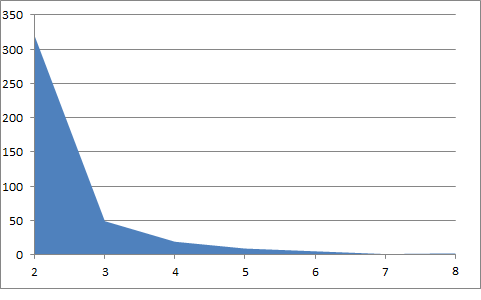
\includegraphics{img/meaningTypePlot2.png}
\caption{Distrubution of number of polysemous types per number of meanings}
\end{figure}


Three types of experiments for each model were performed, in order to tune each model to achieve its 
best performance.
\subsection{Tuning preprocessing parameters}
Each of the preprocessing measures mentioned before 
(lowercasing, filtering words that belong to the closed class group, stemming and merging of lexical
variants in Czech language) was experimented against the different document size (5,3,1 sentence 
document and 3+3, 2+2, 1+1 words surrounding polysemous word) to determine for which parameters the model achieves the highest accuracy. These models were evaluated only for highly polysemous
words, at the fixed size of the evaluation context size. In  order to able to test how models really perform 
we train models only on highly polysemous words, the ones that have 5 or more meanings.  For instance, there are 19 
polysemous words in the test development set that can take 5 to 8 meanings.

\subsection{Tuning evaluation context size} 
When the best parameters for preprocessing and document size (in the term--document matrix) are 
discovered, the next tuning phase experiments with different sizes of Evaluation Context against these best 
paremeters. There are two motivations for this sequence of tuning experiments: first, the preprocessing
 and building the matrix come before matrix frequency normalization and evaluation. Second, after
the best parameters in the preprocessing stage are found, we can observe how this (best) model behaves 
with different sizes of context (from which the evaluation context vector is constructed). 

\subsection{Evaluation on polysemous words of different level } 
Words whose orthographic representation can take on a large number of meanings can be considered
as ''highly polysemous", while words that can take on a small number of meanings(like two or three) can 
be regarded as ''not highly polysemous". As explained, numbers of occurrences of polysemous words 
conform to the Zipfian distribution, which means that there is only a small number of highly polysemous
words. Therefore, when experimenting with such words test set is not overly large, but if other, less
polysemous words are included, the number of test set instances rise. The purpose of this experiment
is to investigate how do models handle more and less polysemous words. Ranges from 2 to 8 meanings per word
are taken into consideration.

\newpage
\section{TF--IDF experiments}
As previously mentioned experiments are organized around 3 different different Vector Space Models, 
based on the weighting of the matrix elements or dimensionality reduction technique. Matrix reduction technique used for this model was TF--IDF (described in Chapter 6.5). For all the models experiments were performed on every parameter for a range of meaningful values. Parameters are grouped according to the phase in which they were used in:
\begin{itemize}
\item Tuning preprocessing parameters (preprocessing method and document size in co-occurrence matrix)
\item Tuning evaluation context size 
\item Evaluation on polysemous words of different level
\end{itemize}
These rounds are ordered sequentially in order to ensure best possible tuning for the model. Final step
represents an evaluation on words with different degree of ambiguity attached to them.

\subsection{Tuning preprocessing parameters}
First, no preprocessing method was applied on the train and test set. The size of the document in the term--document co-
occurrence matrix was changed in order to observe the influence on the precision. A threshold number of meanings to be evaluated on was set to 5, which means that other polysemous words that had less than 5 meanings encountered in training were discarded for this test. There was 177 polysemous words that appeared in 1861 occurrences, and for this test set a number of test instances was discarded for having a 
low number of meanings. The reason for discarding is that this round of tests is aimed at finding the best preprocessing method, so therefore a full number of test instances was not necessary.  
 An evaluation context size was fixed to 3, which means that a symmetric window 3 preceding and 3 succeeding words were used to build a vector which was used for classification. First column in the table displays the preprocessing method used on the entire corpus (except on the test instances) used in the phase of constructing co--occurrence matrix. To ensure that the best preprocessing method is chosen, regardless of the 
document size used in co--occurrence matrix, different size of documents were observed. Document sizes that were
experimented with are: 5 sentence document, 3 sentence document, 1 sentence document, and 3+3, 2+2, 1+1 symmetric word windows around polysemous word.  
For baseline random precision was calculated for every individual test. Random precision represents the precision of the system when it is picking a random meaning for a polysemous word that is tested. 
Precision and recall (in \%) for every document size is presented in the tables below. First a sentence--level 
document size was experimented with. This means that for the units from which the frequencies were calculated from (for the co-occurrence matrix) the paragraphs of size 1, 3 and 5 sentences. 
Best results in all the tables are bolded. 

\begin{table}[h!]
\begin{tabular}{ l | r r | r r | r r | r}
   preprocessing &  1 sentence && 3 sentences && 5 sentences  && random\\
\hline
	& P  &  R & P  &  R & P  &  R & precision\\
\hline\hline
 NO  & 92.31 & 100 & 94.57 & 100 & 95.67 & 100  &11.36 \\
LOWCASE  & 90.6 & 100 & 91.45 & 100 & 92.31 & 100 & 11.36 \\
STOP  & 89.74 & 100 & 93.16 & 100 & 94.87 & 100 & 11.36 \\
 STEM  & 90.6 & 100 & \textbf{96.58} & 100 & 95.73 & 100 & 11.36 \\
 MERGE  & 90.6 & 100 & 94.87 & 100 & 95.72 & 100 & 11.36 \\
\end{tabular}
\caption{Precision and Recall using various individual preprocessing techniques, sentence level document size}
\end{table}

Random precision is the same regardless of the preprocessing technique applied due to the fact that 
they were applied to all tokens except the polysemous words. This had helped preserve the size of the 
test set, which reflected on the consistent number of random precision in tests. Recall is 100 because all test instances were encountered in training and the system was able to
provide an answer. This is not necessarily always the case, it depends on the pseudo--random split on 
training and testing sets  whether an instance will be encountered during training. 
\\\\
It seems that individual 
 preprocessing technique that yields best results is stemming, though lowercasing and merging of Czech variants give the most consistent results. To ensure the validity of these findings, same test was repeated for the word--level document size. Results are given in the table below.  
\begin{table}[h!]
\begin{tabular}{ l | r r | r r | r r | r}
   preprocessing & 1+1 word && 2+2 words && 3+3 words  && random\\
\hline\hline
	& P  &  R & P  &  R & P  &  R &\\
\hline
NO  & 90.6 & 100 & 94.87 & 100 & 95.73 & 100 & 13.96 \\
LOWCASE  & 91.45 & 100 & 95.73 & 100 & 95.73 & 100 & 13.96 \\
 STOP  & 89.74 & 100 & 93.16 & 100 & 94.87 & 100 & 13.96  \\
 STEM  & 90.6 & 100 & 96.58 & 100 & 95.73 & 100 & 13.96 \\
MERGE  & 93.58 & 100 & 98.17 & 100 & \textbf{98.17} & 100 & 13.76  \\
\end{tabular}
\caption{Precision and Recall of TF--IDF model, no preprocessing, word level document size}
\end{table}

Evaluation of preprocessing technique on the word level document size gives approximatively similar results, though it can be observed that merging of Czech variants gives slightly better results in this case. Lowercasing filtering of Czech stop words is not that far behind. In the next round of experiments, combinations of best individual techniques were tested to find out whether an improvement is obtained. 
Results are given in the tables below. 


 \begin{table}[h!]
\begin{footnotesize}
\begin{tabular}{ l | r r | r r | r r | r}
preprocessing & \multicolumn{2}{l|}{1 sentence} & \multicolumn{2}{l|}{3 sentences} & \multicolumn{2}{l|}{5 sentences} & random\\
\hline
	& P  &  R & P  &  R & P  &  R & precision\\
\hline\hline
STOP+LOWCASE  & 90.6 & 100 & 92.31 & 100 & 91.45 & 100 & 13.96\\
 STEM+MERGE  & 91.45 & 100 & 91.45 & 100 & 91.45 & 100 & 13.96 \\
 STEM+LOWCASE  & 91.45 & 100 & 91.45 & 100 & 91.45 & 100 & 13.96 \\
 STOP+MERGE  & 92.31 & 100 & 93.16 & 100 & \textbf{93.16} & 100 & 13.96 \\
STEM+STOP+LOWCASE  & 91.45 & 100 & \textbf{93.16} & 100 & 92.31 & 100 & 13.96 \\
STEM+STOP+MERGE  & 91.45 & 100 & \textbf{93.16} & 100 & 92.31 & 100 & 13.96 \\
STOP+MERGE+LOWCASE  & 90.6 & 100 & 92.31 & 100 & 91.45 & 100 & 13.96 \\
STEM+STOP+& 91.45 & 100 & \textbf{93.16} & 100 & 92.31 & 100 & 13.96 \\
+MERGE+LOWCASE  &&&&&&&\\
\end{tabular}
\caption{Precision and Recall using combinations of preprocessing techniques, sentence level document size}
\end{footnotesize}
\end{table}


It seems that the combination of filters reduces the word space too much, which causes the overall precision to deteriorate a bit. It is also interesting to see that application of combination of 3 techniques yields slightly better results than the application of just 2 techniques. If we look at the last column, where all 4 preprocessing techniques were tested, we can see that results are the same as for the combinations of 3 techniques which do not include merge of Czech lexical variants. It would seem that this technique does not contribute any improvement when in combination with other preprocessing techniques. 

Same combinations were tested out on the word level document size, in order to confirm the findings from the previous table. Results are given in the table below. 
\begin{table}[h!]
\begin{footnotesize}
\begin{tabular}{ l | r r | r r | r r | r}
preprocessing & \multicolumn{2}{l|}{1+1 word} & \multicolumn{2}{l|}{2+2 words} & \multicolumn{2}{l|}{3+3 words} & random\\
\hline\hline
	& P  &  R & P  &  R & P  &  R &\\
\hline
STOP+LOWCASE  & 91.45 & 100 & 94.87 & 100 & 95.73 & 100 & 13.96 \\
STEM+MERGE  & 90.6 & 100 & 96.58 & 100 & 95.73 & 100 & 13.96 \\
STEM+LOWCASE  & 90.6 & 100 & 96.58 & 100 & 95.73 & 100  & 13.96   \\
STOP+MERGE  & 89.74 & 100 & 93.16 & 100 & 94.87 & 100 & 13.96 \\
STEM+STOP+LOWCASE  & 92.31 & 100 & 96.58 & 100 & 95.73 & 100 & 13.96\\
STEM+STOP+MERGE  & 92.31 & 100 & 96.58 & 100 & 95.73 & 100 & 13.96 \\
STOP+MERGE+LOWCASE  & 91.45 & 100 & 94.87 & 100 & 95.73 & 100 & 13.96 \\
STEM+STOP+  & 91.45 & 100 & 94.87 & 100 & 95.73 & 100 & 13.96 \\
+MERGE+LOWCASE  &&&&&&&\\
\end{tabular}
\caption{Precision and Recall of TF--IDF model, no preprocessing, word level document size}
\end{footnotesize}
\end{table}

Experiments on combinations of preprocessing techniques for different word level document sizes showed approximatively the same results as the ones on the sentence level document size. This led to the same 
conclusion as inferred before-- there is a slight improvement in applying 3 or 4 preprocessing techniques, though when compared to applying individual technique the results are still slightly worse . An explanation for this could be that when the word space shrinks too much, TF--IDF weighting becomes to similar for different meanings of tested polysemes, and the algorithm starts to make false predictions.   


Although results achieved without any preprocessing whatsoever are good ones it should be noted that the size of the test set is not that large and that more than 60\% of test set data was 
discarded as unsuitable for this experiment for having to few meanings attached to them. Best achieved result without preprocessing was 
accomplished for 1 sentence document size and 2+2 word window for sentence level and word level document, respectively. Again, the sole purpose of this phase of experiments was to establish which preprocessing method (or combination of methods) is the best one.  

Lowercasing produced a somewhat smaller vocabulary over the entire corpus, which resulted in merging 
several word types. Still, the accuracy of the algorithm was at a very high level.

Filtering words that belong to closed class of words gave the best results out of all preprocessing 
approaches. Precision and recall were at a very high level.
Moreover, it reduced the word space, which considerably influenced the time of computation. If it was to
be compared with the test of the set that was not preprocessed, it can be observed that testing in this 
case was performed 2 times faster. This is viewable from the logs (see User Manual).
Stemming and merging variants produced good results as well, at a high level of test set size. 
All models perform outstanding compared to random prediction. 
\\\\
%\vspace{10 mm}
\textbf{Conclusion.} 
The sole purpose of this round of experiments was to determine the best preprocessing method (or combinations of methods) for the TF--IDF model, for different sizes of document in the co-occurrence matrix. 
First, it can be observed that preprocessing with stemming or merging Czech lexical variants produced the
best results, though filtering of Czech stop words and lowercasing were not far behind. Combination of various preprocessing methods produced somewhat weaker results. This can be explained that after a lot of token merging and cleaning, the word space was for this test data (PDT) overly reduced. As a result, the TDF--IDF weight in term vectors became more similar than before. This prevented the model to perform correct discrimination between all 
meanings of an ambiguous word in a given context.

The last thing which can be observed for all the values of parameters is the document size which 
produced best results. For TF--IDF model a golden middle seems to yield best results, somewhere 
between 1 sentence document, and 3+3 symmetric window around ambiguous word.


\subsection{Tuning evaluation context size}
Evaluation context size is the size of symmetric window of context which is taken into consideration 
when the polysemous word is encountered during prediction of the correct meaning for the word in context. Words that are found within the context
window are used to form a context vector. This context vector's distance is measured against every
vector of each  of the meanings for the polysemous word in question. Sizes of evaluation context size 
experimented with range from 1 to 7. In order to have a larger test set, number of meanings that 
a word can take was lowered to 3 instead of 5 like in the preprocessing experiments.
As concluded in the previous section, best preprocessing methods were stemming and merging (individually), for which the document size was set to 1 sentence, or 3+3 surrounding words, respectively. Therefore they were experimented here with in this phase of tuning. 
Results are given 
in the table below, with best results in bold.

\begin{table}[h!]
\begin{tabular}{ l | r r r r r r r }
    &  1+1 & 2+2 & 3+3 & 4+4 & 5+5 & 6+6 & 7+7 \\
\hline
STEM (1 sentence)  & 93.09 & \textbf{94.69} & 93.93 & 93.47 & 93.02 & 93.02 & 92.87 \\
MERGE (3+3 words) & 93.72 & \textbf{95.26} & 94.84 & 94.69 & 94.99 & 94.99 & 93.93 \\
\end{tabular}
\caption{Precision of TF--IDF model for stemming with document size set to 1 sentence and merge with document size set to 3+3, with various evaluation context sizes}
\end{table} 

Because the same division training and test development set were used as in tuning preprocessing methods Recall was 100\%, and therefore it was not displayed in the table above. 
\textbf{Random precision} for the number of meanings threshold set to 3 was \textbf{20.42\%}. Random precision was higher than in the case of tuning preprocessing methods due to the fact that the number of meaning threshold was lowered which resulted with testing more words that have higher random accuracy. 
\\\\
\textbf{Conclusion.}\\
First thing that can be noticed is that merging of Czech lexical variants, with document size set to 3+3 
neighboring words around ambiguous word outperforms stemming with document size set to 1 sentence, 
for every value of evaluation context size. It is also interesting to observe that for both test cases the best 
evaluation context size is the 2 words surrounding the test word. In the figure below it is observable that 
the precision peaks at around evaluation context size (ECS) set to 2, and then it deteriorates as ECS is increased.
\begin{figure}[h!]
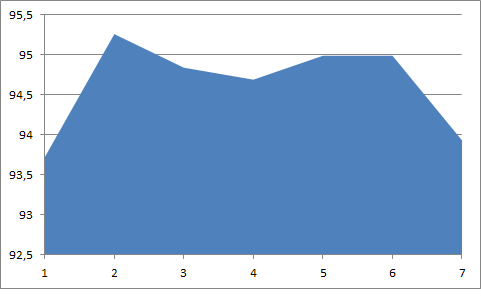
\includegraphics{img/precision-evalContSize_merge.png}
\caption{Precision against evaluation context size, for preprocessing method set to merge of Czech lexical variants and document size set to 3+3}
\end{figure}

 Variance in both sets of results 
is very low, hence there is not much difference in which context size will be used for final evaluation
of all occurrences of polysemous words.


\subsection{ Evaluation on polysemous words of different level}
So far we have been training the model on highly polysemous words, the ones that have 6 or more 
meanings attached to them. Random prediction on these highly polysemous words is very low, therefore
they present a better, more unbiased test set than for instance words that have only 2 meanings, and 
for which random accuracy is 50\%. We will now observe the accuracy of the model set with best
parameters to see how it performs on different sets of words with the same number of meanings. This means
that for instance, in the first column are results of experiments performed on words with 2 meanings attached to them.
Training is performed on the merged set of training and testing development, and testing is done on the unseen set.

\begin{table}[h!]
\begin{tabular}{ l | r r r r r r r  }
     & 2 & 3 & 4 & 5 & 6& 7 & 8  \\
 \hline
Precision  & 92.49 & 97.08 & 87.87 & 97.57 & 64.71 & \textbf{98.49} & 46.15\\ 
Recall & 99.82 & 99.85 & 99.47 & 99.72 & 84.62 & \textbf{99.13} & 60\\ 
Random Precision & 50 & 33.33 & 25 & 20 & 16.67 & 14.29 & 12.5 \\
\end{tabular}
\caption{Precision and Recall of TF--IDF model, closed class filter, document size 1, evaluation context size 3+3 measured against words with different number of meanings}
\end{table} 

\textbf{Conclusion.}\\
We can see that for every group of polysemous words TF--IDF model performs well, where recall is high. The 
lowest scores were noted on words with 6 and 8 meanings, where recall is 84\% and 60\% respectively. Another 
thing that characterizes these low scores is that the test were performed on a low number of instances- there are 
42 instances in the final test set of words with 6 meanings, and only 10 instances of words with 8 meanings. In all other cases number of instances was exceeding 500 test instances, which makes their results a more reliable estimator of the model's accuracy. Precision is reasonably high for all and though it would be expected to be lower 
for words with more meanings, like in the case of words with 7 meanings, out of 508 test instances only 11 were misclassified which resulted with the highest precision on this test set, of  98.49\%.

Overall, it can be said that TF--IFD model performed well at this task. 

\newpage
\section{PMI experiments} 
Experiments with PMI model are like the ones with TF--IDF, grouped in three rounds in order to tune
the model for the best performance. PMI weighting should increase sensitivity of the word to its correct context. 
The theory behind PMI is explained in Chapter 5.4.3.
\begin{itemize}
\item Tuning preprocessing parameters
\item Tuning evaluation context size
\item Evaluation on polysemous words of different level
\end{itemize}
These rounds are ordered sequentially in order to ensure best possible tuning for the model. Final step
represents an evaluation on words with different degree of ambiguity attached to them.


\subsection{Tuning preprocessing parameters}
Being that reasons for using certain values for preprocessing methods parameters were thoroughly described in 
previous section it will not be done again here. From tuning the preprocessing 
parameters for TF--IDF we have a general idea which values for document sizes and preprocessing 
methods give best values. We will thus be concentrating on a smaller set of values for preprocessing parameters. 
Results will be given in summed tables for all preprocessing methods, measured against different 
document sizes.  Other parameters are fixed like in TF--IDF tuning experiments: 
evaluation context size is set to 3, which means that a symmetric window 3 preceding and 3 succeeding words were used to build a vector which was used for classification. The threshold number of meanings was set to 5, which means that every word with the number of sense attached to them that is lower or equal to 5 is discarded from the evaluation. Like before, first was experimented with the individual preprocessing methods. 
Below are given tables for the document size of sentence level. Best results in all the tables are given in bold. 
\begin{table}[h!]
\begin{tabular}{ l | c c | c c | c c | c}
   preprocessing &  1 sentence && 3 sentences && 5 sentences  && random\\
\hline
	& P  &  R & P  &  R & P  &  R &\\
\hline\hline
NO  & 92.31 & 100 & 94.83 & 100 & 95.27 & 100 &  13.96 \\
LOWCASE  & \textbf{98.01} & 100 & 95.01 & 100 & 95.17 & 100 & 13.96  \\
STOP  & 92.31 & 100 & 94.72 & 100 & 93.86 & 100 & 13.96 \\
STEM  & 91.45 & 100 & 91.45 & 100 & 91.45 & 100 & 13.96\\
MERGE  & 92.31 & 100 & 94.83 & 100 & 95.27 & 100 & 13.96 \\
\end{tabular}
\caption{Precision and Recall of PMI model, individual preprocessing methods, sentence level document size}
\end{table}

Total number of not--discarded test set instances was 1174. Random precision was the same for all test cases, as 
was recall (100\%). It seems that lowercasing produced the best result. All other individual preprocessing 
methods achieved slightly better (like the Czech stop word filtering), or slightly worse results (stemming) than with when no preprocessing method was applied to the training set. It is interesting to see that merging of Czech variants brought no improvement whatsoever. Same tests were repeated for the word level document size.

\begin{table}[h!]
\begin{tabular}{ l | c c | c c | c c | c}
   preprocessing &  1+1 word && 2+2 words && 3+3 words && random\\
\hline
	& P  &  R & P  &  R & P  &  R &\\
\hline\hline
NO  & 90.6 & 100 & 94.87 & 100 & 95.73 & 100 & 13.96 \\
LOWCASE  & 94.47 & 100 & \textbf{97.49} & 100 & 97.41 & 100 & 11.47  \\
STOP  & 89.74 & 100 & 93.16 & 100 & 94.87 & 100 & 13.96 \\
STEM  & 90.6 & 100 & 96.58 & 100 & 95.73 & 100 & 13.96\\
 MERGE  & 90.6 & 100 & 94.87 & 100 & 95.73 & 100 & 13.96 \\
\end{tabular}
\caption{Precision and Recall of PMI model, individual preprocessing methods, word level document size}
\end{table}

In the next round of experiments designed for tuning, combinations of preprocessing methods were experimented 
with. First the combinations of methods were tried, for different values of sentence level for document size.
 \begin{table}[h!]
\begin{small}
\begin{tabular}{ l | c c | c c | c c | c}
preprocessing & \multicolumn{2}{l|}{1 sentence} & \multicolumn{2}{l|}{3 sentences} & \multicolumn{2}{l|}{5 sentences} & random\\
\hline
	& P  &  R & P  &  R & P  &  R & precision\\
\hline\hline
 STEM+LOWCASE  & \textbf{98.01} & 100 & 97.93 & 100 & \textbf{98.01} & 100 & 11.47\\
STOP+MERGE  & 92.31 & 100 & 94.72 & 100 & 93.86 & 100 & 13.02 \\
STOP+MERGE+LOWCASE  & 97.84 & 100 & 95.56 & 100 & 94.24 & 100 &11.47\\
STEM+STOP+& 97.93 & 100 & 97.93 & 100 & \textbf{98.01} & 100 & 11.47 \\
+MERGE+LOWCASE  &&&&&&&\\
\end{tabular}
\caption{Precision and Recall using combinations of preprocessing techniques, sentence level document size}
\end{small}
\end{table}

It seems that the combination of more preprocessing methods achieves an increase in accuracy with the PMI model. Also, It would appear that merging of Czech lexical variants does not contribute in this combination of 
methods. Contrary to it, combinations where lowercasing appears seem to be giving good results. Lowercasing proved its mettle in individual tests of preprocessing methods. Then the same test cases were repeated, only this time for the document size word level values. The reason why 
these test cases are repeated is to validate the findings from the previous table. 

 \begin{table}[h!]
\begin{small}
\begin{tabular}{ l | c c | c c | c c | c}
preprocessing & \multicolumn{2}{l|}{1+1 word} & \multicolumn{2}{l|}{2+2 words} & \multicolumn{2}{l|}{3+3 words} & random\\
\hline
	& P  &  R & P  &  R & P  &  R & precision\\
\hline\hline
STEM+LOWCASE  & 95.68 & 100 & \textbf{97.93} & 100 & 97.93 & 100 & 11.47\\
STOP+MERGE  & 89.74 & 100 & 93.16 & 100 & 94.87 & 100 & 13.96 \\
STOP+MERGE+LOWCASE  & 93.95 & 100 & 97.06 & 100 & 97.06 & 100 & 11.47\\
STEM+STOP+ & 95.25 & 100 & 97.93 & 100 & 97.67 & 100 & 11.47 \\
+MERGE+LOWCASE  &&&&&&&\\
\end{tabular}
\caption{Precision and Recall using combinations of preprocessing techniques, word level document size}
\end{small}
\end{table}


It can be observed that best results for the PMI weighted model are achieved when applying lowercase 
transformation on training and test sets (with the exception of ambiguous words), at the document size set to 
symmetric window of size 3. Test set size was fixed at 1913 instances, out of which 1072 were tested. 
Lowercasing was established to be the best individual preprocessing method (98\% accuracy at the 13\% random 
accuracy, with document size set to 1 sentence). Also in combination with stemming it yielded very good results 
(97.9\& at 12\% random accuracy). With the PMI model, there is general conclusion that combination of 
preprocessing methods actually gives better results. It seems that with reduction of the word space, PMI weights 
become better discriminators of context, when the cosine distance is measured against ambiguous word and its 
context.  

\subsection{Tuning evaluation context size}
Evaluation context size is the size of symmetric window of context which is taken into consideration 
when the polysemous word is encountered during testing. Words that are found within that context
window are used to form a context vector. This context vector's distance is measured against every
vector of each  of the meanings for the polysemous word in question. Sizes of context vector 
experimented with range from 1 to 7. In order to have a larger test set, number of meanings that 
a word can take was lowered to 5 instead of 6 like in the preprocessing experiments. Preprocessing
performed was lowercasing of words, and document size was set to 1 sentence. 
Results are given 
in the table below, and the best result is given in bold. 

\begin{table}[h!]
\begin{tabular}{ l | r r r r r r r}
    &  1+1 & 2+2 & 3+3 & 4+4 & 5+5 & 6+6 & 7+7 \\
\hline
LOWCASE  & 95.54 & 97.75 & \textbf{98.01} & 97.93 & 97.93 & 97.93 & 97.93 \\
\end{tabular}
\caption{Precision and Recall of PMI model,  combined preprocessing methods, word level document size}
\end{table} 

Recall is 100\% for all test cases, therefore it was not displayed in the table. Random prediction is also the same. 
It can be observed that the best evaluation context size is 3+3, and that after it peaks at that point it converges to a stable value for all wider evaluation contexts. 

\textbf{Conclusion.}\\
PMI achieved also very good scores. The best preprocessing method was lowercasing, at 1 sentence document size. The best evaluation context size was found to be 3+3 neighboring words. 


\subsection{ Evaluation on polysemous words of different level}
We will now observe the accuracy of the model set with best
parameters to see how it performs on different sets of words with the same number of meanings. This means
that for instance, in the first column are results of experiments performed on words with 2 meanings attached to them.
Training is performed on the merged set of training and testing development, and testing is done on the unseen set.
\begin{table}[h!]
\begin{tabular}{ l | r r r r r r r  }
     & 2 & 3 & 4 & 5 & 6  \\
 \hline
Precision  & 92.17 & 87.39 & 64.85 & 76.77 & 94.55\\ 
Recall & 99.81 & 99.22 & 98.17 & 95 & 96.3\\ 
Random Precision & 50 & 33.33 & 25 & 20 & 16.67 \\
\end{tabular}
\caption{Precision and Recall of PMI model, lowercase preprocessing , document size 1, evaluation context size 3+3 measured against words with different number of meanings}
\end{table} 

PMI model also achieves nice results for all groups of ambiguous terms with different number of meanings. 

\textbf{Conclusion.}\\
It can be seen that PMI model does not provide predictable results when observed while testing on different levels
of ambiguity. For instance, in the Table 6.16 it can be seen that F--measure seems to deteriorate with the number of meanings 
attached for a word starting from 2, but that it jumps again with words that have 6 meanings. 

Overall, it can be said that TF--IFD model performed well at this task. 



\section{RI experiments} 
Random Indexing experiments were performed in order to see how does the matrix reduction influence on the overall accuracy of the algorithm. No weighting was applied on the co--occurrence matrix. The efficacy of the RI to retrieve semantically similar words is very high. 
 The incentive for applying a matrix reduction technique on the WSD task was that the representation of the ambiguous word as a random vector could actually be close in the vector space to a familiar context, that is context in which it often appears. On the other hand, the algorithm should produce low scores for the target word against an unfamiliar context. 
Experiments  with RI model are also, grouped in three rounds in order to tune
the model for the best performance. In the end best model is evaluated on ambiguous words with 
different counts of meanings attached to them.
\begin{itemize}
\item Tuning preprocessing parameters
\item Tuning evaluation context size
\item Evaluation on polysemous words of different level
\end{itemize}

What is different with RI model is that term--document matrix is built incrementally, by adding initially 
assigned pseudo-random vectors of documents to initially pseudo-random vectors of terms. No 
weighting is applied to elements of the matrix. Matrix itself is of much less dimensionality than the 
standard co-occurrence matrix, and is also much less sparse (considerably lower count of zero 
elements). 
 Dimension of random vectors is preset before the construction of matrix and in our 
experiments has that value of 300.

\subsection{Tuning preprocessing parameters}
Like with the models tested before different document sizes and preprocessing methods were tunned
for the best performance of the RI model. 

\begin{table}[h!]
\begin{tabular}{ l | r | r | r | r}
   preprocessing &  5 sentences & 3 sentences & 1 sentence  & random\\
\hline
	& P  &  P  &  P  &  \\
\hline\hline
 NO  & 69.21  & 70.73  &71.1 & 13.6 \\
LOWCASE  &72.4 & 73.52 & 74.54 &13.6   \\
CLOSED CLASS &70.76 & 72.52 & 76.37 &13.6   \\
STEM+MERGE & 71.5 & 72.21 & 74.19 & 13.6   \\
\end{tabular}
\caption{Precision and Recall of RI model, various preprocessing methods, sentence level document size}
\end{table}

Recall and random prediction were the same for all document sizes, hence they were not displayed in the table above. This aggregated table shows both individual and combined preprocessing methods. Same test cases were 
repeated for the document size of word level. 

\begin{table}[h!]
\begin{tabular}{ l |  r | r | r | r}
   preprocessing &  3+3 words& 2+2 words& 1+1 word& random\\
\hline
	& P  &  P  &  P  &  \\
\hline\hline
NO &  71.36 & 72.51 & 74.37  & 13.6\\
LOWCASE  &72.4 & 73.52 & 74.54 &13.6   \\
CLOSED CLASS & 76.85 &77.33 &78.45 & 13.6\\
STEM+MERGE   & 73.71  & 75.2 & 76.84 &13.6\\
\end{tabular}
\caption{Precision and Recall of RI model, various preprocessing methods, word level document size}
\end{table}


It seems that for RI model smaller document size produces better results. The reason for that can be found in the very nature of term vector generation in RI. Term vectors are constructed from 
superposition of all document vectors it appears in. Document vectors are initially sparse vectors, which
means that the smaller the document size is, the stronger relation gets between a word and its context.
The best model achieved 76.84\% accuracy, with a 100\% Recall, for document size set to 1+1 context
window, and preprocessing method set to filtering of closed--class words.

\subsection{Tuning evaluation context size}
Evaluation context size is the size of symmetric window of context which is taken into consideration 
when the polysemous word is encountered during testing. Words that are found within that context
window are used to form a context vector. This context vector's distance is measured against every
vector of each  of the meanings for the polysemous word in question. Sizes of context vector 
experimented with range from 1 to 7. In order to have a larger test set, number of meanings that 
a word can take was lowered to 5 instead of 6 like in the preprocessing experiments. Preprocessing
performed was lowercasing of words, and document size was set to 1 sentence. 
Results are given 
in the table below, and the best result is given in bold. 

\begin{table}[h!]
\begin{tabular}{ l | r r r r r r r}
    &  1+1 & 2+2 & 3+3 & 4+4 & 5+5 & 6+6 & 7+7 \\
\hline
CLOSED CLASS  & 80.16 & 85.14 & \textbf{86.74} & 79.54 & 79.54& 79.54& 79.54\\
\end{tabular}
\caption{Precision and Recall of RI model,  combined preprocessing methods, word level document size}
\end{table} 

Recall is 100\% for all test cases, therefore it was not displayed in the table. Random prediction is also the same. 
It can be observed that the best evaluation context size is 3+3, and that after it peaks at that point it converges to a stable value for all wider evaluation contexts. 



\subsection{Evaluation on polysemous words of different level}
The best model is evaluated on ambiguous words with 
different counts of meanings attached to them.

\begin{table}[h!]
\begin{tabular}{ l | r r r r r r}
     & 2 & 3 & 4 & 5 & 6& 7     \\
 \hline
Precision & 87.4 & 86.02 & 84.19 & 76.41 &80.5 & 45.48 \\
Recall   & 95.44 & 98.48 & 94.71 & 95.12 & 100.0 &100.0    \\
Random prediction    & 50 & 33.33 & 25 & 20 & 16.66 & 14.28      \\
\end{tabular}
\caption{Precision and Recall of RI model, closed class filter, document size 1+1, evaluation context size 3+3 measured against words with different number of meanings}
\end{table} 
 It is observable that the best score is achieved with the words that have 3 meanings, but from there precision falls down. It is 
just 45\% for the words with 7 meanings attached to them. Out of all models tested, Random Indexing has the poorest 
performance. One possible explanation is that too much of a contextual information is lost when matrix reduction of the co--
occurrence matrix is performed. As outlined before RI performs well in tasks with the paradigmatic use of context, like in the 
individual word similarity task. However when employed in the WSD task the algorithm is calculating the cosine similarity between the test 
context and all sense candidates for an ambiguous word, where term vectors are extracted from a co-occurrence matrix which has reduced dimensionality. 
It seems that level of contextual information which is vital for the WSD task is lowered as well with the RI matrix reduction, which leads to the poorer performance of the algorithm. 

\chapter{Implementation}
Software used in all the experiments in this thesis is developed under the name PDT Word Sense Disambiguator. Entire system was implemented in Java programming language. Two third--party libraries were used: 
\begin{enumerate}
\item lucene\footnote{http://lucene.apache.org/java/docs/index.html}: for the purpose of text indexing,  released under the Apache Software License and
\item semantic vectors\footnote{http://code.google.com/p/semanticvectors/}: for the purpose of constructing random vectors, released under the BSD 2-Clause License   \footnote{http://www.opensource.org/licenses/bsd-license.php}
\end{enumerate}
Classes are separated into following packages: preprocessing, vectorModels, utils (contains data types, string manipulation classes, vector operation classes), evaluation and experiments. 

\section{Data flow}
In this section will be presented an outline of sequential steps taken by the system in order to train the
model, and then evaluate it on the test set. The options  mentioned here are dicussed in length in previous chapters,  therefore I will 
outline here only what is relevant for the data flow.There are 4 major stages that subsume a number of 
smaller, potential steps:
\begin{description}
\item \textbf{Obtaining and dividing the data} \hfill \\
	First step here is to extract the text from PDT1.0(which is in a form of fully annotated SGML text). 
Different meanings of ambiguous word are annotated differently, so this information is kept, while all
other words are extracted in their normal form. This part is vital because the model needs to be trained
on different meanings in order to be able to differentiate them during testing. 
	When the text is obtained it is divided into three sets: training, testing for development and final testing. Sentences from 
original data set are randomized before division. Training takes about 9/10 of the entire data set, while 1/10 is evenly 
distributed to remaining two sets. Evaluation is performed twice: during training, the model is trained 
on training set, and tested to development test set.  During testing, model is trained on train+testDev 
set and evaluated on final test set, which represents an unseen portion of data. Files that are trained on
and later tested on are run through the indexer. Every vector used in experiments is built straight from 
the indexer. 
\item \textbf{Preprocessing} \hfill \\
There are 4 preproccessing options (all optional): lowercasing, stemming, filtering words that belong to closed class,
and merging Czech lexical variants.  Lowercasing and word filtering take place in the indexer: lowercasing is just a matter of option, while for word filtering a stop word list needs to be passed. This list is to be found in the Apendix 1. Stemming and merging of czech variants are performed by the program directly on files. If one of these two options is used, it is applied before indexing.  
\item \textbf{Building the matrix}\hfill \\
After preprocessing indexer builds co-occurrence matrix (term--document). Documents passed to the 
indexer are determined by the system, and there are two options that can be set: number of sentences 
in one index document, and size of the context window found around ambiguous word. Any positive number can be set on either option, there is just a rule not to set number of sentences to a value 
larger than 1 when you want to build word--level documents. Choice of document size determines 
the "sensitivity" of the model, as is dicussed in Experiments chapter. During this phase all meanings of
ambiguous word are saved in the hash table. Elements of the hash table are items whose keys are 
ambiguous words while the values attached to the keys are lists which keep all the 
meanings of ambiguous word. This hash table is passed to evaluator during evaluation. 
\item \textbf{Normalizing the matrix: frequency weighting or dimensionality reduction }\hfill \\
Although in case of frequency weighting this step is performed during evaluation, it is more natural to
come before it, therefore I will describe it here. Frequency weighting is performed on elements of 
term--document matrix, and which weight scheme is applied depends on the model (either TF--IDF or 
PMI). Weighting is however not applied to RI model, due to its nature (see chapter on Random Indexing). RI model is constructed with the usage of semantic vectors package. After this step, the model is considered to be trained, and is ready for the evaluation.
\item  \textbf{Evaluation}\hfill \\
Evaluation is performed in several steps. First the entire test set is passed in order to extract all the 
ambiguous words and the contexts they are found in. For some reason in PDT1 some words are labeled
as ambiguous although they have only one meaning. These kinds of occurrences are inserted in 
previously mentioned hash table during matrix construction phase. If a an ambiguous word encountered 
in testing is determined to have only one meaning in training, it is not put into the test set. 
When test set instances are extracted, model compares distances between a test set instance of 
ambigous word and all other meanings to the context vector. Whichever meaning is the closest by 
cosine distance from the context vector is predicted to be the ''correct meaning". Term vectors are retrieved at this point, and in the case of TFIDF and PMI they are weighted on the spot. RI were
created during indexing and stored in $termvectors.bin$ file.   
\end{description}
\chapter{User manual}
In this section it will be explained how to use the software developed for the purpose of the experiments. First section describes the parameters 

\section{Input parameters}
System is accessed through a single class to which command line parameters are passed in the form:
\begin{center}
[-argumentType   argumentValue]*
\end{center}

\textbf{Class to which the arguments should be passed is  called $Experiment$.  }

All arguments are optional. All arguments have their default values. Class that parses arguments is called $Arguments$.
An overview of all input arguments is given in the table below.

\begin{table}[h!]
\begin{footnotesize}
\begin{tabular}{| l|c|c|c|c|}
\hline
   index  &  name & data type & default value & used for  \\
\hline\hline
	1  &  lowercase & String & "n"  & preprocessing \\ \hline
	2  &  stopWordsRemoval & String & "n"  & preprocessing \\ \hline
	3  &  stemming & String & "n"  & preprocessing \\ \hline
	4  &  mergeLexicalVariants & String & "n"  & preprocessing \\ \hline
	5  &  inputFilePath & String & pdt1\_cleaned  & getting data \\ \hline
	6  &  numberOfSentencesInLuceneDoc & Integer & 1  & document size \\ \hline
	7  &  numberOfWordsInDocument & Integer & -1  & document size \\ \hline
	8  &  matrixType & Integer & 0  & \small{\{0,1,2\}=\{TFIDF,PMI,RI\}} \\  \hline
	9  &  upBoarderForNumberOfMeanings & Integer & 6  & evaluation \\ \hline
	10  &  evaluationContextWindowSize & Integer & 3  & evaluation \\ \hline
\hline
\end{tabular}
\caption{Overview of system's input arguments}
\end{footnotesize}
\end{table}

If someone wishes to perform WSD on another dataset, they should specify the path to the file with the
$-inputFilePath$ argument. However, it should be noted that occurrences of polysemous words should
be annotated so that different meanings could be differentiated by the system. Content of the file
 passed to the system is split into three separate files: train, testDev, testFinal. TestFinal contains test
test sentences. 


\section{Logs}
For every experiment a log is made in the log folder, containing all relevant statistics related to the 
experiment. Log name is constructed from abbreviations of all values of experiment's phases, for instance: $PMI\_STOP+MERGE\_1s\_7w\_6m$ means that it is a log of PMI model, where in preprocessing
 filtering out closed class words and merging lexical variants was performed, document size in term--doc matrix is 1 sentence, 7+7 evaluation window context was used to construct context vectors, and only words with 6 meanings were investigated.
%\chapter*{Z�v�r}

\chapter*{Conclusion}
The primary task of this Master's thesis was to perform Word Sense Disambiguation on the Prague 
Dependency Treebank dataset. A single methodology was crafted and applied to three different semantic models to ensure an objective comparison between the two models which perform TF--IDF and PMI weighting of the co-occurrence matrix, and one model which performs dimensionality reduction of the same matrix. This methodology served to tune the 
models and find which preprocessing technique, document size and evaluation context size produce best results. 
Results, though achieved on a different data set, are comparable to some of the state--of--the--art approaches form the Senseval/Semeval competitions. There are other approaches like(Yarowsky et. al 2001) that similarly to this approach use the cosine similarity to assign the word to its correct sense (in this case a centroid).However their approach is different
in the way the classification is performed. Further more, it has not been attempted so far to employ RI on the WSD task, to the best of author's knowledge. 
Major conclusion of this thesis is that the models that do not perform matrix reduction on the co-occurrence matrix outperform the approach that does (in this case Random Indexing). Another fact that appears to be the same for all three models is that the size of the document in the term--document matrix that helps produce the best results of the algorithm is 3+3 symmetric context around the polysemous word. It seems that when training with the document concentrated around polysemous word a model becomes more sensitive to such contexts and is ultimately a better discriminator in the evaluation.

\addcontentsline{toc}{chapter}{Summary}



\appendix


\bibliography{myrefs}{
\addcontentsline{toc}{chapter}{Bibliography}
}
\bibliographystyle{plainnat}


%\chapwithtoc{List of Tables}
\listoftables
%\chapwithtoc{List of Abbreviations}

\chapwithtoc{Appendices}
\chapter{List of filter words for Czech language}
Below is given a list of Czech stop words, consisting of words that belong to closed class words, and some frequent words that are assessed to carry little contextual information. More detail description on stop--word filtering can be found in Chapter 5.1.
\\\\\
[dnes cz
timto budes
budem byli jses muj  svym ta tomto  tohle tuto tyto jej  zda  proc  mate  tato  kam  tohoto  kdo  kteri
mi   nam  tom  tomuto  mit   nic  proto kterou byla toho protoze asi ho nasi napiste re coz tim takze
svych  jeji svymi jste  aj tu tedy teto bylo kde ke prave ji  nad nejsou ci pod tema mezi  pres  ty
pak vam  ani kdyz vsak  ne jsem tento clanku clanky aby jsme pred pta jejich byl jeste az bez take
pouze  prvni vase ktera nas novy tipy pokud muze design strana  jeho sve jine zpravy nove neni	vas
jen   podle  zde clanek uz email byt vice bude jiz nez  ktery by  tere  co nebo ten tak  ma pri
od po jsou jak dalsi ale si ve to jako za zpet  ze  do  pro  je 
na]

\openright

\end{document}
